\pdfoutput=1
\documentclass[11pt]{amsart}
\usepackage{amsmath,amssymb,amsthm}
\usepackage[margin=1.2in]{geometry}
\usepackage{booktabs,adjustbox,xcolor,graphicx}
\usepackage[colorlinks=true,linkcolor=blue,citecolor=blue,urlcolor=blue]{hyperref}
\hypersetup{pdfauthor={Bernd Johannes Wuebben},
pdftitle={All-time approximation of Hermitian--Yang--Mills flow on degenerating curves}}
\setlength{\emergencystretch}{2em}
\newtheorem{theorem}{Theorem}[section]
\newtheorem{proposition}[theorem]{Proposition}
\newtheorem{lemma}[theorem]{Lemma}
\newtheorem{corollary}[theorem]{Corollary}
\theoremstyle{definition}
\newtheorem{definition}[theorem]{Definition}
\newtheorem{example}[theorem]{Example}
\theoremstyle{remark}
\newtheorem{remark}[theorem]{Remark}
\newcommand{\RR}{\mathbb R}
\newcommand{\CC}{\mathbb C}
\newcommand{\PP}{\mathbb P}
\newcommand{\cC}{\mathcal C}
\newcommand{\cP}{\mathcal P}
\newcommand{\cF}{\mathcal F}
\newcommand{\cR}{\mathcal R}
\newcommand{\cN}{\mathcal N}
\newcommand{\Herm}{\operatorname{Herm}}
\newcommand{\tr}{\operatorname{tr}}
\newcommand{\Ad}{\operatorname{Ad}}
\newcommand{\End}{\operatorname{End}}
\newcommand{\Geo}{\operatorname{Geo}}
\newcommand{\SU}{\operatorname{SU}}
\newcommand{\HS}{\mathrm{HS}}
\newcommand{\grad}{\operatorname{grad}}
\newcommand{\dist}{\operatorname{dist}}
\newcommand{\supp}{\operatorname{supp}}
\title[All-time HYM approximation]{All-time approximation of Hermitian--Yang--Mills flow on degenerating curves}
\author{Bernd Johannes Wuebben}
\subjclass[2020]{53C07 (primary); 14D06, 58J35, 58J50 (secondary)}
\keywords{Hermitian--Yang--Mills flow, nodal degeneration, flat bundle,
small eigenvalue, matrix gradient flow, gluing}
\date{November 11, 2026\\This version: November 11, 2026}

\begin{document}
\begin{abstract}
We prove an all-time approximation of Hermitian--Yang--Mills flow by a
finite matrix gradient flow on a degenerating family of compact genus-three
curves. Four independent node parameters and two component-holonomy
parameters determine flat unitary bundles passing from stable to strictly
polystable. With fixed infinitesimal holonomy generators and node
identifications, the spatially integrated squared error is bounded,
uniformly in time, by the initial integrated trace discrepancy plus an
error vanishing as all six parameters tend independently to zero.
Actual initial metrics are uniformly bounded and finite initial data lie
in a small ball; no lower bound on the weakest decay rate is required.
An open spatial initial class enters after preparation negligible on every
finite relaxation scale. The proof writes the first-order component-frame
error as a global divergence using its zero angular mean, and combines
HYM energy with time-integrated bounds from the finite gradient flow.
We also prove relative asymptotics for every positive small eigenvalue of
the endomorphism connection Laplacian, with exact correspondence of kernels
and varying node identifications. One stable family has relaxation scales
of orders $h^{-1}$, $h^{-2}$ and $h^{-4}$ as $h\to0$, all covered by
the nonlinear theorem.
\end{abstract}
\maketitle
\section{Introduction}\label{sec:introduction}

Hermitian--Yang--Mills flow on a degenerating curve can have several
relaxation scales. Long annuli weaken the interaction between normalization
components, while a component connection approaching a reducible connection
introduces further small endomorphism modes. An approximation on a fixed
multiple of the shortest annular length need not reach the time at which
the weakest mode relaxes. The problem is to compare actual trajectories
with a finite matrix evolution on the entire positive time axis, allowing
these two sources of small eigenvalues to vary independently.

We consider a compact genus-three plumbing family with two elliptic and
two rational normalization components. Four independent node parameters
control the annular lengths. Two independent real parameters control flat
unitary connections on the elliptic components. Fixed unitary identifications
at the nodes give a flat bundle on the entire family; its component and
cycle holonomies can be noncommuting. The finite configuration space is a
product of spaces of positive Hermitian matrices of determinant one. Its
potential is the sum of component commutator potentials and squared
distances across the nodes, with their geometrically determined weights.

The all-time comparison uses two different estimates for the error of the
reconstructed metric. The component and radial errors have an integrable
bound in terms of the finite forces. The first-order change from component
frames to parallel node frames has only the first angular Fourier modes.
A Neumann problem on each incidence collar writes this error as a
divergence whose space-time energy is small. The actual HYM energy identity
then controls its contribution to the trace comparison. This argument does
not divide by the smallest positive eigenvalue.

Throughout the all-time theorem, the component matrices and node
identifications are fixed. Only their nonnegative weights vary, and the
initial finite metrics lie in a specified small ball. Zero component
weights and nonzero common kernels are permitted. The approximation is an
absolute integrated squared-distance estimate; it does not compare errors
relative to a trajectory that is tending to zero.

\subsection{The main theorem}
Let $C_\tau$ be the smooth fibre of the four-node family constructed
in Section~\ref{sec:geometry}. Its normalization components have
area one. On the elliptic components the reference connections are
$d-i\alpha_iT_i\vartheta_i$, where $T_i$ are fixed trace-free
Hermitian matrices and $\vartheta_i$ fixed nonzero real harmonic
one-forms. The rational component connections are trivial.
The parameters $\alpha_i$ are real and independent of the four
complex node parameters $\tau_e\ne0$. Write $h_0$ for the
global parallel bundle metric and set
\[
 L_e=\log(1/|\tau_e|),\quad L_*=\min_eL_e,\quad
 \epsilon_e=L_e^{-1},\quad
 \alpha_*=\max_i|\alpha_i|,\quad
 \kappa_i=\int_{E_i}|\vartheta_i|^2.
\]
The joint limit is $\alpha_*\to0$ and $L_*\to\infty$.
All parameters are held constant during each flow.

Let $\cP_r$ be the positive determinant-one Hermitian matrices,
with metric $\langle V,W\rangle_H=\tr(H^{-1}VH^{-1}W)$
and distance $d$. Equip $\cP_r^4$ with the product metric
$g_A$ weighted by the component areas $A_i=1$.
The finite evolution is the negative gradient flow of
\begin{equation}\label{eq:intro-potential}
 \Phi(H)=
 \sum_{i=+,-}\alpha_i^2\kappa_i
   \{\tr(T_iH_i^{-1}T_iH_i)-\tr(T_i^2)\}
 +\pi\sum_{e=ij}\epsilon_e d(H_i,U_{ij}H_jU_{ij}^*)^2.
\end{equation}
Its matrix equation is printed in \eqref{eq:finite-flow}.
The determinant-one actual HYM equation is
$h^{-1}\partial_sh=-2i\Lambda F_h$ in physical time $s$.
For two metrics define
$D_{\tr}(h,k)=\tr(h^{-1}k+k^{-1}h-2I)$.

\begin{theorem}\label{thm:intro}
Fix the rank, component metrics, matrices $T_i$, harmonic forms
$\vartheta_i$ and unitary node identifications $U_e$. There
is $R_*>0$ and an explicit smooth reconstruction
$H\mapsto\widehat K_{\tau,\alpha}(H)$ such that the following
holds for sufficiently small joint parameters.
Let $H(s)$ be the finite gradient flow from distance at most
$R_*$ from $(I,I,I,I)$. Let $h(s)$ be actual HYM flow on
the same smooth fibre, from any smooth metric with the parallel
determinant and fixed bounds $ch_0\le h(0)\le C_0h_0$.
Then
\begin{equation}\label{eq:intro-main}
 \sup_{s\ge0}\int_{C_\tau}
     d(h(s),\widehat K_{\tau,\alpha}(H(s)))^2\,dA_\tau
 \le\eta+C\left(\alpha_*+
                   \frac{(1+\log L_*)^2}{L_*}\right),
\end{equation}
where
$\eta=\int_{C_\tau}D_{\tr}(h(0),\widehat K_{\tau,\alpha}(H(0)))\,dA_\tau$.
Constants are independent of all $\alpha_i^2L_e$,
all $L_e/L_f$, and time. Component weights may vanish and
the common space of parallel trace-free endomorphisms may
be nonzero. On each fixed compact normalization region the
reconstruction differs from $H_i(s)$ by $O(L_*^{-1})$.
\end{theorem}

The proof is Theorem~\ref{thm:all-time}. The exponentially
small geometric-transfer term in \eqref{eq:all-time-error}
is absorbed in the error displayed here. Uniform approximation
requires $\eta\to0$ over the chosen initial family.
Theorem~\ref{thm:spatial-entry} removes the need to prescribe
the finite initial tuple. It gives a nonempty open class of
spatially varying smooth metrics, defined by the component
extension norm \eqref{eq:extension-norm}, which enters the
comparison at a common time $s_*\to\infty$ satisfying
$(\alpha_*^2+L_*^{-1})s_*\to0$. The selected tuple depends
on the initial component profiles. Smooth middle-neck data
need only obey the fixed pointwise bound; their derivatives
need not be bounded uniformly.

Theorem~\ref{thm:relative-spectrum} identifies every small
eigenvalue of the actual endomorphism connection Laplacian.
Its finite energy is the sum of
$\alpha_i^2\kappa_i\|[T_i,X_i]\|^2$ and
$(2\pi/L_e)\|X_i-\Ad(U_e)X_j\|^2$, with mass
$\sum_i A_i\|X_i\|^2$. The comparison is relative for
every positive weak eigenvalue, identifies the exact kernel,
and leaves a uniform complementary gap. In contrast to the
all-time nonlinear constants, this spectral result is uniform
also when the transports vary through reducible tuples.

The same family contains a stable rank-two example with
three node weights $h$, a fourth node weight $h^2$, and
component weight $\alpha_+^2\kappa_+=h^4$. Its twelve
small eigenvalues comprise nine order-$h$ modes, two
asymptotic to $\tfrac12h^2$, and one asymptotic to $h^4$.
Corollary~\ref{cor:three-scales} proves both these spectral
claims and actual nonlinear approximation through $h^{-4}$
and all later times. The latter conclusion uses the all-time
residual argument, independently of the spectral asymptotics.

\subsection{The analytic mechanism}
The reconstruction uses scalar component Green functions,
exactly flat geodesic node profiles and relative-logarithm
interpolation on collars of radius $\rho=L_*^{-1}$.
The frame change on an elliptic incidence is
$e^{i\alpha_iT_iF_{ie}}$ with $F_{ie}$ a real linear
harmonic function in the branch coordinate. Estimating its
cutoff error in absolute $L^1$ can produce an integral
of size $1/|\alpha_i|$; the explicit calculation
\eqref{eq:first-order-divergence} explains this difficulty.

Instead, the term linear in $\alpha_i$ in the full Chern
expression has only angular Fourier indices $1,-1$ after
the conformal area factor is removed. Its entrywise zero
mean allows a collar Neumann solve with zero normal trace
at both boundaries. Extension by zero gives a global
divergence without a boundary measure. Thus the residual is
$D^*J+B$, with $J$ small in space-time $L^2$ and $B$ small
in space-time $L^1$. The trace comparison pairs $J$ with
derivatives of the actual and reconstructed metrics; both
have uniformly bounded total energy.

For the remainder $B$, a fixed-matrix weighted normal
equation estimate controls the separate finite forces by
the gradient on a small ball. Ohta's bounded-image
rectifiability theorem for self-contracted curves
\cite{ohta} then gives their uniform total integral.
The fixed-constraint restriction enters at this step.
The matrix counterexample in Section~\ref{sec:finite}
shows why a uniform lower bound for the full unweighted
matrix alone does not suffice.

\subsection{Relation to earlier work}
Burger's theorem gives relative scalar graph asymptotics
on hyperbolic surfaces with unrestricted ratios among
the short geodesic lengths \cite{burger}. Ji--Wentworth
prove spectral convergence for conic degenerations
\cite{ji-wentworth,ji-wentworth-correction}; their
correction replaces a false isoperimetric lemma, which
is not used here. Daskalopoulos--Wentworth establish
connection-valued spectral convergence and uniform
Yang--Mills estimates away from accidental reducibility
\cite[Theorem~4.13, Corollary~4.14 and
Proposition~5.8]{dw}. Our normalization components carry
reducible holonomy, so their uniform-gap argument does
not supply the additional slow dynamics considered here.

Haiden--Katzarkov--Kontsevich--Pandit develop
finite-dimensional asymptotic descriptions of HYM flow
on a fixed base \cite{hkkp}. Their Proposition~4.5
also compares exact and approximate metrics under an
integrable pointwise bound on the forcing. The
divergence estimate here uses spatially integrated
energy to treat a first-order collar term not controlled
uniformly under degeneration by that pointwise criterion.
Lam's fixed-base asymptotic
theorem for semistable bundles assumes a locally free
graded bundle, with additional rationality hypotheses
in its detailed reduction \cite{lam}. Applying these
results fibre by fibre does not give constants uniform
under pinching.

Previous work on nodal curves gives actual
noncommuting HYM approximation on bounded slow-time
intervals \cite{wuebben-effective} and treats
nontrivial gluing, spatial entry and all-time
comparison under a positive normalized rate
\cite{wuebben-gluing}. The present result removes
that rate requirement for fixed constraints on a
small basin and couples independent node and
component-holonomy scales in one compact family.
The new all-time step is the global divergence
decomposition of the full Chern residual; the
finite graph operator or the scalar multiscale
principle alone is not that step.

\section{A compact family with independent parameters}\label{sec:geometry}

We first construct the compact family and fix the gauges used in the
analysis. The construction is classical pointed plumbing
\cite[\S8.3]{hubbard-koch}, with a particular choice of component metrics
and flat connections. The auxiliary markings will be forgotten without
contracting any component.

\subsection{The curve and its metrics}
Let $E$ be the smooth projective completion of
\[
 y^2=(x-1)(x-2)(x-3),
\]
and let $p,q$ be the two points over $x=0$. Take copies $E_+,E_-$ of
$E$ and copies $R_p,R_q$ of $\PP^1$. Join the two points named $p$ to
$0,\infty$ on $R_p$, and join the two points named $q$ to $0,\infty$
on $R_q$. The resulting nodal curve $C_0$ has dual graph $K_{2,2}$.
Its arithmetic genus is $1+1+1=3$. The points $1\in R_p,R_q$ make it a
stable two-pointed curve.

Choose disjoint coordinate disks at all eight branch points, using flat
coordinates on the elliptic curves and unitary M\"obius coordinates on
the rational curves. With the components and these coordinates fixed,
pointed plumbing gives a proper flat family
\begin{equation}\label{eq:plumbing}
 \pi:\cC\longrightarrow B=\Delta_\delta^4,
 \qquad u_ev_e=\tau_e\quad(e\in E(K_{2,2})).
\end{equation}
Here $E(K_{2,2})$ denotes the edge set, not the elliptic curve. All four
$\tau_e$ are independent. For clarity, choose fixed radii $0<a<b_0$
in the coordinate disks and $\delta<a^2$. The product component exteriors
are glued to the patches $|u_e|,|v_e|<b_0$ by
\[
 (u_e,\tau)\longmapsto
 (u_e,\tau_e/u_e,\tau_{f\ne e}),
\]
and the analogous map on the other branch. The two incidence overlaps of
one node are disjoint, since both $|u_e|>a$ and $|v_e|>a$ would imply
$|\tau_e|>a^2$. Different node patches are disjoint. There are no triple
incidence overlaps. Locally the total space has coordinates
$(u_e,v_e,\tau_{f\ne e})$ and is smooth. Every fibre with all
$\tau_e\ne0$ is a connected smooth compact curve of genus three.
Forgetting the two sections leaves the same proper family. In particular,
the rational bridges in $C_0$ remain present. Independence of these family
parameters makes no assertion about injectivity into unmarked moduli.

\begin{figure}[htbp]
\centering
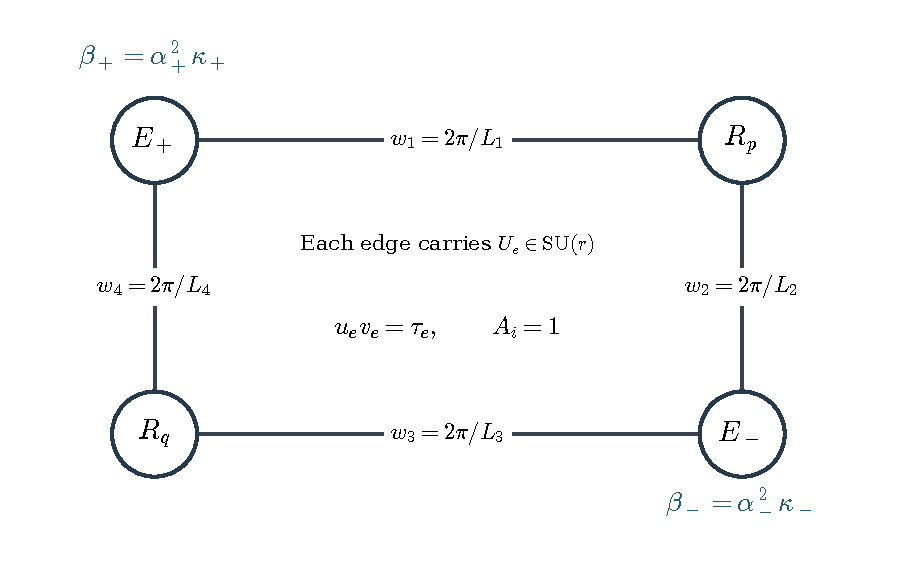
\includegraphics[width=\textwidth]{figures/output/fig02_family.pdf}
\caption{The four normalization components and their independent
parameters. The edge coefficients are $w_e=2\pi/L_e$ and the two
component coefficients are $\beta_i=\alpha_i^2\kappa_i$. The
rational bridges are retained in the compact family.}
\label{fig:family}
\end{figure}

Give $E_+,E_-$ their flat metrics of area one and $R_p,R_q$ their
Fubini--Study metrics of area one. Write $\omega_i^{\mathrm{area}}$ for
these K\"ahler forms and $A_i=1$ for their areas.

\begin{lemma}\label{lem:total-metric}
After shrinking $B$, the total space $\cC$ has a smooth K\"ahler form
whose restriction to each central normalization component is
$\omega_i^{\mathrm{area}}$. Each smooth fibre has area four. On a
sufficiently small node patch its fibre metric is the restriction of
$\omega_i^{\mathrm{area}}(u_e)+\omega_j^{\mathrm{area}}(v_e)$.
\end{lemma}

\begin{proof}
Choose on each component a degree-one holomorphic line bundle $L_i$ with
a Hermitian metric of Chern form $\omega_i^{\mathrm{area}}$. On an
elliptic component, start with any metric on a degree-one line bundle and
solve the scalar Poisson equation for the difference of the two curvature
forms. That difference has integral zero. Fourier series on the flat
torus give a smooth solution. On $\PP^1$, take $\mathcal O(1)$.
We use the convention in which a degree-one Chern form integrates to one.

In a holomorphic frame near a branch point write the squared norm as
$e^{-\psi_i(u)}$, with $\psi_i(0)=0$. On an elliptic branch a
holomorphic frame change removes the harmonic part of the potential,
leaving a positive multiple of $|u|^2$. On a rational branch the chosen
coordinate gives a positive multiple of $\log(1+|u|^2)$. In particular,
the first derivative of every $\psi_i$ vanishes at zero.

Glue the product line bundles on the component exteriors to a trivial
line on each node patch by these frames. The absence of triple incidence
overlaps verifies the cocycle condition. On a smaller node patch set the
squared norm of its frame equal to
\[
 \exp\{-\psi_i(u_e)-\psi_j(v_e)\}.
\]
On the $u_e$ overlap its ratio to the component metric is
$\exp\{-\psi_j(\tau_e/u_e)\}$. Interpolate the logarithm of this
ratio on a fixed incidence collar, leaving the product metric unchanged
outside it. The resulting smooth metric on the line bundle has Chern
form $\Omega$. Along a central branch the correction and all its
tangential derivatives vanish, so its restriction is exactly the
prescribed component form. On the smaller node patches its curvature is
the sum of the two branch forms.

Let $\omega_B$ be the Euclidean form on $B$. Near a node,
$\Omega+C\pi^*\omega_B$ is positive for every $C>0$: the branch
forms control the $u_e,v_e$ directions and the base form controls the
remaining three coordinates. On the compact remainder of the central
fibre, $\pi$ is a submersion and $\Omega$ is strictly positive on the
vertical tangent. In finitely many submersion charts, a Schur-complement
estimate makes $\Omega+C\pi^*\omega_B$ positive for one sufficiently
large $C$. Properness and a smaller $B$ make these neighborhoods cover
every fibre. The form is closed and of type $(1,1)$, hence K\"ahler.
Its fibre restrictions do not depend on the added base form. The degree
of the line bundle on every smooth fibre is $\sum_i\deg L_i=4$.
\end{proof}

Write $dA_\tau$ for this fibre area form and define
\begin{equation}\label{eq:parameters}
 L_e=\log(1/|\tau_e|),\quad L_* =\min_e L_e,\quad
 \epsilon_e=L_e^{-1},\quad \epsilon_* =L_*^{-1},\quad
 b=\max_e|\tau_e|=e^{-L_*}.
\end{equation}
All limits below have $L_*\to\infty$.

\begin{lemma}\label{lem:geometric-estimates}
Choose a radius $\rho$ with $b<\rho^2$. The middle annulus of node
$e$, given by $|\tau_e|/\rho<|u_e|<\rho$, has area at most
$C\rho^2$, independently of its modulus. Its scalar Dirichlet capacity
is
\begin{equation}\label{eq:capacity}
 \frac{2\pi}{L_e+2\log\rho}.
\end{equation}
The punctured component $|u_e|\ge\rho$ has a natural holomorphic
identification with its image in $C_\tau$. For every fixed derivative
order $m$, its fibre metric differs from the component metric by at most
$C_m b^2\rho^{-N_m}$ in that order, for some finite $N_m$.
\end{lemma}

\begin{proof}
The two branch terms in Lemma~\ref{lem:total-metric} each integrate
over a disk of radius $\rho$, proving the area bound. In complex
dimension one the Dirichlet integral is conformally invariant. The
radial harmonic function between the two boundary circles is affine in
$\log|u_e|$, and direct integration of its squared derivative gives
\eqref{eq:capacity}. In the branch identification, $v_e=\tau_e/u_e$.
Differentiating this identity in the fixed branch potentials gives the
stated polynomial losses in $\rho^{-1}$ and the factor $|\tau_e|^2$.
On the fixed interpolation collars the denominators are bounded, and
outside them the metric agrees with the product metric. No inverse power
of an individual $\tau_e$ occurs. In particular $\rho=L_*^{-1}$
makes every required error tend to zero.
\end{proof}

\subsection{The flat bundle}
Fix $r\ge2$, trace-free Hermitian matrices $T_+,T_-$, and nonzero real
harmonic one-forms $\vartheta_+,\vartheta_-$ on the two flat elliptic
curves. For two small real numbers $\alpha_+,\alpha_-$ set
\begin{equation}\label{eq:component-connection}
 D_i=d-i\alpha_iT_i\vartheta_i\quad(i=+,-),
 \qquad D_i=d\quad(i=p,q),
 \qquad \kappa_i=\int_{E_i}|\vartheta_i|^2\,dA_i.
\end{equation}
The elliptic connections are expressed in global smooth unitary frames.
Their curvature and determinant connection vanish. Near an elliptic
branch point the primitive of $\vartheta_i$ vanishing at the point is
\begin{equation}\label{eq:primitive}
 F_{ie}(u)=c_{ie}^{\mathrm{harm}}u+
           \overline{c_{ie}^{\mathrm{harm}}u}.
\end{equation}
This identity is exact: the coordinates are flat and the harmonic
one-form is constant. The change of frame
$G_{ie}=\exp(i\alpha_iT_iF_{ie})$ is unitary and gives a parallel
frame. On rational branches put $G_{ie}=I$.

Fix unitary matrices $U_{ij}\in\SU(r)$ on oriented edges, with
$U_{ji}=U_{ij}^{-1}$. We use the convention that they carry the
$j$-end data to the $i$-end frame. Glue a trivial flat bundle on each
node patch to the component local systems using constant identifications
in these parallel frames, with relative matrix $U_{ij}$.

\begin{proposition}\label{prop:bundle-family}
For every fixed $\alpha=(\alpha_+,\alpha_-)$ these identifications
define a flat unitary connection $D$ and parallel determinant on a
holomorphic vector bundle over the whole smooth total space $\cC$.
They depend smoothly on $\alpha$. The four complex parameters $\tau_e$
and the two real parameters $\alpha_i$ vary independently. The parallel
Hermitian metric $h_0$ restricts to an HYM metric of slope zero on every
smooth fibre.
\end{proposition}

\begin{proof}
Pull each component connection back to its product exterior, taking the
full exterior derivative there. It is flat. On every incidence overlap,
the designated frames are parallel, and the constant node
identifications are isomorphisms of flat connections. There are no
triple incidence overlaps. The connections and metrics therefore glue.
Flatness implies $(D^{0,1})^2=0$, so local parallel frames are
holomorphic and define the asserted locally free bundle on $\cC$.
All transition maps have determinant one. This construction uses no
relation between $\alpha$ and $\tau$ and depends smoothly on the real
parameters. We assert holomorphic dependence on $\tau$ for each fixed
$\alpha$, not a flat connection in the additional real parameter
directions. The fibrewise Chern curvature of $h_0$ vanishes.
\end{proof}

\subsection{Stability and parallel endomorphisms}
Shrinking the allowed $\alpha$ interval once, the parallel trace-free
Hermitian endomorphisms of $D$ are exactly the tuples satisfying
\begin{equation}\label{eq:common-kernel}
 X_i=\Ad(U_{ij})X_j\quad(e=ij),\qquad
 \alpha_i[T_i,X_i]=0\quad(i=+,-).
\end{equation}
Indeed, choose a nonzero period of $\vartheta_i$. For sufficiently small
nonzero $\alpha_i$, distinct eigenvalues of $T_i$ remain distinct
after exponentiation by that period. Its holonomy commutant is thus the
commutant of $T_i$. A commuting endomorphism is constant in the harmonic
gauge and in each node-normalized parallel frame. Node compatibility is
precisely the first equation of \eqref{eq:common-kernel}. When
$\alpha_i=0$ the second equation is vacuous.

The unitary-flat correspondence \cite{narasimhan-seshadri} makes every
smooth-fibre bundle polystable of degree zero. It is stable exactly when
\eqref{eq:common-kernel} has no nonzero solution. Equivalently, the
degree formula for a holomorphic subbundle expresses its degree as the
negative squared norm of its second fundamental form. Equality forces a
parallel orthogonal splitting. Conversely a nonzero trace-free Hermitian
commutant supplies such a splitting by its eigenspaces.

For an explicit transition in rank two, let
\begin{equation}\label{eq:pauli-data}
 T_+=\sigma_z=\begin{pmatrix}1&0\\0&-1\end{pmatrix},\qquad
 \alpha_-=0,\qquad
 U=\frac{I+i\sigma_x}{\sqrt2},\qquad
 \sigma_x=\begin{pmatrix}0&1\\1&0\end{pmatrix}.
\end{equation}
Take the identity on a spanning tree and $U$ on the remaining edge.
Tree compatibility makes all $X_i$ equal. For $\alpha_+\ne0$, the
component commutant is the $\sigma_z$ axis, whereas the cycle edge
fixes the $\sigma_x$ axis. Their intersection is zero. At
$\alpha_+=0$ the latter axis survives. Thus the same compact family is
stable for sufficiently small $\alpha_+\ne0$ and strictly polystable
at $\alpha_+=0$.

The component and cycle operations in this example do not commute.
To interpret cycle holonomy, fix basepoints and paths to the nodes.
The resulting based holonomy includes component path factors
$\exp(i\alpha_iT_i\int\vartheta_i)$ as well as the $U_{ij}$.
A product of node matrices alone is not generally the based holonomy.
The family changes holomorphic stability by changing the bundle, not
by changing the polarization of a curve. Its underlying smooth
$\SU(r)$ bundle is topologically trivial; no unstable locus is
claimed.

\section{The finite evolution and its total force}\label{sec:finite}

Let $\cP_r$ be the space of positive Hermitian $r\times r$ matrices
of determinant one. Its affine-invariant metric is
\[
 \langle V,W\rangle_H=\tr(H^{-1}VH^{-1}W),
 \qquad
 d(H,K)=\|\log(H^{-1/2}KH^{-1/2})\|_{\HS}.
\]
It is a finite-dimensional Hadamard manifold. On $\cP_r^4$ use the
product metric $g_A=\sum_i A_i g_i$ and write $o=(I,I,I,I)$.
The masses are $A_i=1$ in our family; retaining them in the formulas
indicates the origin of each coefficient. All matrix norms below are
Hilbert--Schmidt norms unless stated otherwise.

For a Hermitian matrix $T$ set
\begin{equation}\label{eq:component-potential}
 f_T(H)=\tr(TH^{-1}TH)-\tr(T^2).
\end{equation}
On the family of Section~\ref{sec:geometry} define
\begin{equation}\label{eq:potential}
 \Phi(H)=\sum_{i=+,-}\alpha_i^2\kappa_i f_{T_i}(H_i)
       +\pi\sum_{e=ij}\epsilon_e d(H_i,U_{ij}H_jU_{ij}^*)^2.
\end{equation}
The negative gradient equation is
\begin{equation}\label{eq:finite-flow}
 H_i^{-1}\dot H_i
 =-\frac{\alpha_i^2\kappa_i}{A_i}
       [T_i,H_i^{-1}T_iH_i]
  +\frac{2\pi}{A_i}\sum_{e=ij}\epsilon_e B_{ij},
 \qquad B_{ij}=\log(H_i^{-1}U_{ij}H_jU_{ij}^*).
\end{equation}
The component term is omitted at rational vertices. The logarithm in
$B_{ij}$ is the principal matrix logarithm; it is $H_i$-self-adjoint
and trace-free. The edge summation uses the orientation from the vertex
under consideration. To check the component term, vary $H$ by $HX$,
with $X$ $H$-self-adjoint and trace-free. Differentiating
\eqref{eq:component-potential} gives
\[
 df_T(H)[HX]=\tr\bigl([T,H^{-1}TH]X\bigr).
\]
The gradient of half the squared distance to $K$ is
$-H\log(H^{-1}K)$, giving the edge term. The later reconstruction
derives the same coefficients from the Chern equation on the compact
fibre.

The following finite estimate is useful because it has no dependence
on a smallest positive weighted eigenvalue. We prove it on an arbitrary
fixed graph, allowing several component matrices at a vertex.

\begin{theorem}\label{thm:finite-force}
Fix a finite graph with $N$ vertices, rank $r\ge2$, positive masses
$A_i$, unitary edge matrices $U_e$, and a finite list of Hermitian
matrices $T_a$ at vertices $i(a)$. For arbitrary constant nonnegative
weights $w_e,\beta_a$ put
\begin{align}
 \Phi_{w,\beta}(H)&=\frac12\sum_e w_e
       d(H_i,U_eH_jU_e^*)^2+\sum_a\beta_a f_{T_a}(H_{i(a)}),
       \label{eq:general-potential}\\
 \cF_{w,\beta}(H)&=\sum_e w_e d(H_i,U_eH_jU_e^*)
           +\sum_a\beta_a\sqrt{2f_{T_a}(H_{i(a)})}.
       \label{eq:force}
\end{align}
There are $R_*>0$ and $c,C>0$, depending only on the fixed data,
such that, on $d_A(H,o)\le R_*$,
\begin{equation}\label{eq:force-gradient}
 c\cF_{w,\beta}(H)\le
 \|\grad\Phi_{w,\beta}(H)\|_{g_A}
 \le C\cF_{w,\beta}(H).
\end{equation}
The negative gradient trajectory starting at distance $R\le R_*$
exists for all $s\ge0$, stays in that ball, and satisfies
\begin{equation}\label{eq:force-integral}
 \int_0^\infty\bigl(\cF_{w,\beta}(H(s))
                   +\|\dot H(s)\|_{g_A}\bigr)\,ds\le CR,
 \qquad
 \int_0^\infty\Phi_{w,\beta}(H(s))\,ds\le\frac12R^2.
\end{equation}
It converges to a minimizer. These constants are independent of all
weights, their ratios and the subset of weights that vanish.
\end{theorem}

\subsection{A weighted linear estimate}
The elementary ingredient is a formula for a weighted least-squares
left inverse. Its constant retains the geometry of the fixed rows.

\begin{lemma}\label{lem:weighted-matrix}
For every fixed real matrix $D$ there is $C_D<\infty$ such that
\begin{equation}\label{eq:weighted-matrix}
 \|WDx\|\le C_D\|D^TWDx\|
\end{equation}
for every nonnegative diagonal matrix $W$ and every $x$.
\end{lemma}

\begin{proof}
First suppose $D$ is an $m\times n$ matrix of full column rank and
$W$ is positive. Let $D_S=R_SD$ be its restriction to $n$ rows, and
let $\mathfrak B$ consist of the subsets for which $\det D_S\ne0$.
Set $G=D^TWD$. Cauchy--Binet gives
\[
 \det G=\sum_{|S|=n}\det(D_S)^2\prod_{j\in S}w_j.
\]
In particular the numbers
\[
 p_S=\frac{\det(D_S)^2\prod_{j\in S}w_j}{\det G}
 \quad(S\in\mathfrak B)
\]
are nonnegative and sum to one. Replacing column $k$ of $D$ by $y$
replaces column $k$ of $D^TWD$ by $D^TWy$. Cauchy--Binet for this
replacement, followed by Cramer's rule, gives
\begin{equation}\label{eq:weighted-left-inverse}
 G^{-1}D^TW=\sum_{S\in\mathfrak B}p_S D_S^{-1}R_S.
\end{equation}
Terms with singular $D_S$ already vanish before Cramer's rule is
applied. Each $R_S$ has norm one, so the norm of
\eqref{eq:weighted-left-inverse} is at most
$\max_{S\in\mathfrak B}\|D_S^{-1}\|$. Transposing and applying
the result to $Gx$ proves \eqref{eq:weighted-matrix}.

For a matrix of rank $p>0$, choose an isometry $Q:\RR^p\to\RR^n$
onto $(\ker D)^\perp$. Apply the preceding argument to $D'=DQ$.
The identities $D=D'Q^T$ and $D^T=Q(D')^T$ preserve the norm on
the right of \eqref{eq:weighted-matrix}. Finally replace $W$ by
$W+\delta I$ and let $\delta\downarrow0$. This limit uses the
inequality, not an inverse of a singular normal matrix. The case $D=0$
is immediate.
\end{proof}

If $D$ is divided into $J$ fixed blocks $D_k$ and $W$ has constant
weight $\lambda_k\ge0$ on each block, the lemma gives
\begin{equation}\label{eq:linear-force}
 F^0(x):=\sum_k\lambda_k\|D_kx\|
 \le\sqrt J\,C_D\|D^TWDx\|.
\end{equation}
The choice of $(\ker D)^\perp$ is made once for the full fixed
matrix. It does not change with the support of $W$.

\subsection{Exact zero sets and nonlinear absorption}
Use real coordinates $x_i=\sqrt{A_i}\log H_i$. Then
$|x|=d_A(H,o)$ and the pullback metric is Euclidean at zero. The
linear edge maps and component maps are
\[
 D_ex=\frac{x_i}{\sqrt{A_i}}-
       \Ad(U_e)\frac{x_j}{\sqrt{A_j}},
 \qquad
 C_ax=i[T_a,x_{i(a)}/\sqrt{A_{i(a)}}].
\]
Both maps take values in real spaces of Hermitian matrices. Associate
to an edge the function $f_e=\frac12d(H_i,U_eH_jU_e^*)^2$, and
to a component matrix the function $f_a=f_{T_a}(H_{i(a)})$.
The exact zero set of $f_e$ is $\ker D_e$, and its Hessian at zero
is $D_e^TD_e$.

For the component assertion, diagonalize $S=\log H$ with eigenvalues
$s_b$. In this basis $T$ is Hermitian and direct multiplication gives
\begin{equation}\label{eq:cosh-potential}
 f_T(e^S)=2\sum_{b<c}|T_{bc}|^2
            \bigl(\cosh(s_b-s_c)-1\bigr)
 \ge\frac12\|[T,S]\|^2.
\end{equation}
Its exact zero set is $[T,S]=0$, and its quadratic term is
$\frac12\|[T,S]\|^2$. Thus the component Hessian is $C_a^TC_a$.
Stack all these maps into $D$. Denote any one block by $D_k$ and
its associated function by $f_k$. Every $f_k$ is nonnegative,
vanishes precisely on $\ker D_k$, and has Hessian $D_k^TD_k$ at
zero. In particular its gradient vanishes on the whole kernel.

On the auxiliary ball $|x|\le1$ the third derivatives of this finite
collection of functions are bounded. Put
$r_k(x)=\nabla f_k(x)-D_k^TD_kx$. On $|x|\le R\le1$,
$\|Dr_k(x)\|\le C_0R$. If $P_k$ is orthogonal projection onto
$\ker D_k$, then $r_k(P_kx)=0$ and the segment from $P_kx$ to
$x$ stays in the ball. Therefore
\begin{equation}\label{eq:block-remainder}
 \|r_k(x)\|\le C_0R\dist(x,\ker D_k)
                \le C_1R\|D_kx\|.
\end{equation}
The last constant uses only the positive singular values of each
nonzero fixed block. Zero blocks can be omitted. Combining
\eqref{eq:block-remainder} with \eqref{eq:linear-force}, and writing
$K=\sqrt J C_D$, gives
\[
 F^0(x)\le K\|\nabla\Phi_{w,\beta}(x)\|
                    +KC_1R F^0(x).
\]
Choose $R_*$ so that $KC_1R_*\le\frac12$. Absorption gives
$F^0\le2K\|\nabla\Phi_{w,\beta}\|$ uniformly in the weights.

For edges, the distance-decreasing logarithm at the identity and the
bounded differential of the exponential on this ball imply
$\|D_ex\|\le\sqrt{2f_e(x)}\le C\|D_ex\|$.
For components, the lower bound is \eqref{eq:cosh-potential}; Taylor
expansion along the segment from $P_ax$ to $x$, on which the initial
function and gradient vanish, gives the upper bound. Hence
$F^0\le\cF_{w,\beta}\le CF^0$. Smooth equivalence of the
coordinate metric with the Euclidean metric proves the left side of
\eqref{eq:force-gradient}. The block bounds
$\|\nabla f_k\|\le C\|D_kx\|$ prove the right side.

\subsection{Convexity and finite length}
To verify geodesic convexity of $f_T$, write
$H(t)=H_0^{1/2}e^{tK}H_0^{1/2}$ and diagonalize the Hermitian matrix
$K$ with eigenvalues $k_b$. For $B=H_0^{-1/2}TH_0^{1/2}$,
\[
 \tr(TH(t)^{-1}TH(t))
       =\sum_{b,c}|B_{cb}|^2 e^{t(k_b-k_c)}.
\]
Each summand is convex. Squared distance between two moving geodesics
is convex on a Hadamard manifold, and unitary conjugation is an
isometry. Thus \eqref{eq:general-potential} is geodesically convex,
nonnegative and minimized at $o$. Its negative gradient flow obeys
\begin{equation}\label{eq:finite-energy}
 \frac12\frac{d}{ds}d_A(H(s),o)^2\le-\Phi_{w,\beta}(H(s)).
\end{equation}
It stays in the compact ball of radius $R$ and exists for all time.
Integration gives the second estimate of \eqref{eq:force-integral}.

For $T>s$, convexity and decreasing potential similarly give
\[
 \frac12\frac{d}{ds}d_A(H(s),H(T))^2
       \le\Phi_{w,\beta}(H(T))-\Phi_{w,\beta}(H(s))\le0.
\]
The curve is therefore self-contracted: its distance to any later
point decreases as its earlier time increases. We apply Ohta's
bounded-image length estimate on a finite-dimensional Hadamard
manifold \cite[Theorem~3.3 and (3.8)]{ohta}. Here the dimension is
$N(r^2-1)\ge3$, the image has diameter at most $2R$, and its
radius-one neighborhood lies in $B(o,R_*+1)$, whose volume is fixed.
The length estimate consequently gives
$\int_0^\infty\|\dot H\|_{g_A}\,ds\le CR$.
Together with \eqref{eq:force-gradient}, this proves the first
estimate of \eqref{eq:force-integral}.

Finite length implies convergence to a point $H_\infty$ in the ball.
If its gradient were nonzero, continuity would give a positive lower
bound for the speed for all sufficiently large times, a contradiction.
Convexity makes $H_\infty$ a global minimizer, so all terms with
positive weights vanish there. In logarithm coordinates the minimizer
set is exactly $\bigcap_{\lambda_k>0}\ker D_k$. The limit need
not be $o$, and the theorem gives neither a uniform rate nor an
explicit formula for this selected limit. This completes the proof
of Theorem~\ref{thm:finite-force}.

\subsection{Dependence on the fixed constraints}
The fixed-matrix hypothesis cannot be replaced by uniform injectivity
of the full matrix. For $\delta>0$ take
\[
 D_\delta=\begin{pmatrix}1&0\\0&1\\1&\delta\end{pmatrix},
 \quad W_\delta=\operatorname{diag}(1,\delta^4,1),
 \quad x_\delta=\begin{pmatrix}-\delta/2\\1\end{pmatrix}.
\]
Although $D_\delta^TD_\delta\ge I$,
\[
 W_\delta D_\delta x_\delta
 =(-\delta/2,\delta^4,\delta/2)^T,
 \qquad D_\delta^TW_\delta D_\delta x_\delta
 =(0,\delta^2/2+\delta^4)^T.
\]
Their norm ratio is asymptotic to $\sqrt2/\delta$.
A row basis that can dominate the weighted normal matrix becomes
singular. This is an obstruction to a uniform force estimate, not
an obstruction theorem for actual HYM approximation.

There is a second distinction needed in the analytic proof. A
component force is weighted by $\alpha^2$, whereas a change of
component frame can have a first-order factor $\alpha$. With one
vertex, mass one, $T=\sigma_z$, $\kappa=1$ and
$H=\exp(q\sigma_x)$, direct calculation gives
\[
 f_T(H)=4\sinh^2q,\qquad
 g(\partial_qH,\partial_qH)=2,\qquad
 \dot q=-2\alpha^2\sinh(2q).
\]
For $q(0)=q_0>0$ and $\alpha>0$ it follows that
\begin{equation}\label{eq:first-order-divergence}
 \int_0^\infty\alpha q(s)\,ds
   =\frac1{2\alpha}\int_0^{q_0}\frac{q}{\sinh(2q)}\,dq.
\end{equation}
The right-hand integral is finite and strictly positive. Thus a
first-order frame error cannot be integrated uniformly by
Theorem~\ref{thm:finite-force} alone. The angular divergence
construction below addresses precisely this term.

\section{HYM comparison with a divergence residual}\label{sec:comparison}

This section applies to any closed Riemann surface $C$ with a fixed
K\"ahler metric and any flat unitary bundle $(E,D,h_0)$ with parallel
determinant metric. A Hermitian metric is represented by a positive
$h_0$-self-adjoint endomorphism. The connection $D$, its formal adjoint
$D^*$, and the norms of endomorphism-valued forms always use this fixed
reference metric. Local parallel unitary frames have constant unitary
transition maps.

\subsection{The Chern equation and its trace inequality}
With area form $dA=a(z)\,dx\,dy=(i/2)a(z)\,dz\wedge d\bar z$, put
$\Delta=-4a^{-1}\partial_z\partial_{\bar z}$, the nonnegative
scalar Laplacian. The equation
\begin{equation}\label{eq:hym}
 h^{-1}h_s=-2i\Lambda F_h
\end{equation}
in a local parallel holomorphic frame is
\begin{equation}\label{eq:local-hym}
 h_s=4a^{-1}(h_{z\bar z}-h_{\bar z}h^{-1}h_z),
 \qquad
 2i\Lambda F_h=-4a^{-1}\partial_{\bar z}(h^{-1}h_z).
\end{equation}
In real coordinates it reads
\begin{equation}\label{eq:real-hym}
 \begin{split}
 ah_s={}&h_{xx}+h_{yy}-h_xh^{-1}h_x-h_yh^{-1}h_y\\
        &+i(h_xh^{-1}h_y-h_yh^{-1}h_x).
 \end{split}
\end{equation}
The last, Hermitian commutator term is retained throughout the proof.
For $h(x,y)=e^{xV+yW}$ at the origin, with noncommuting Hermitian
$V,W$, the first four terms cancel and this term is $i[V,W]$.
Thus \eqref{eq:hym} is not ordinary harmonic-map heat flow into
$\cP_r$.

For smooth positive initial data, the classical compact-base HYM
existence theorem gives a smooth solution for every finite time
\cite{donaldson}; a precise arbitrary-initial-metric statement
and continuation proof are in \cite[Theorem~6.8.25]{kobayashi}.
The book uses time $t=2s$ in our normalization; the statement
in \cite[\S4.1, following (4.8)]{hkkp} uses the normalization
above. The scalar equation for $\log\det h$
preserves the parallel determinant. The maximum principle applied to
$v^*hv$ for a constant local vector $v$ gives the upper order bound:
the quadratic term in \eqref{eq:local-hym} is nonpositive after this
pairing. For $h^{-1}$ the inverse derivative formula gives
\[
 (h^{-1})_s=4a^{-1}\bigl((h^{-1})_{z\bar z}
              -(h^{-1})_z h(h^{-1})_{\bar z}\bigr),
\]
which gives its upper bound as well. Hence
\begin{equation}\label{eq:order-bounds}
 ch_0\le h(0)\le C_0h_0
 \quad\Longrightarrow\quad
 ch_0\le h(s)\le C_0h_0\quad(s\ge0).
\end{equation}
These order comparisons are global and independent of spatial
derivatives of the initial metric. Existence is asserted separately
on each fixed compact smooth fibre; no uniform high-derivative
continuation theorem on degenerating fibres is needed.

Define the trace distance and the residual of a comparison metric by
\begin{equation}\label{eq:trace-residual}
 D_{\tr}(h,K)=\tr(h^{-1}K+K^{-1}h-2I),
 \qquad
 \cR(K)=K^{-1}K_s+2i\Lambda F_K.
\end{equation}
If the eigenvalues of $h^{-1}K$ are $e^{b_j}$, then
\begin{equation}\label{eq:distance-trace}
 d(h,K)^2=\sum_j b_j^2
       \le\sum_j(e^{b_j}+e^{-b_j}-2)=D_{\tr}(h,K).
\end{equation}
On a fixed bounded positive range the reverse inequality holds with
a fixed constant.

\begin{lemma}\label{lem:forced-trace}
For an exact solution $h$ and any smooth comparison metric $K$,
\begin{equation}\label{eq:forced-trace}
 (\partial_s+\Delta)D_{\tr}(h,K)
 \le\operatorname{Re}\tr\bigl((h^{-1}K-K^{-1}h)\cR(K)\bigr).
\end{equation}
\end{lemma}

\begin{proof}
First take two exact flows. At a specified point and time choose a
time-independent holomorphic frame normal for $h$, so $h=I$ and
$\partial h=0$ at that point. Substitution of the Chern equation
into the time derivative and scalar Laplacian of $\tr(h^{-1}K)$
cancels the curvature terms. The remaining expression is
$-4a^{-1}\tr(K_{\bar z}K^{-1}K_z)\le0$. Interchanging the two
metrics proves the inequality for the inverse trace. For a forced
comparison, its extra velocity is $K\cR(K)$. Its contributions to
these two traces are respectively
$\tr(h^{-1}K\cR(K))$ and $-\tr(\cR(K)K^{-1}h)$.
This proves \eqref{eq:forced-trace}. The real part is redundant for
the actual residual because $K\cR(K)$ is Hermitian; retaining it
allows complex pieces in a decomposition of that residual. The
calculation is invariant under changes of holomorphic frame and so
defines a global scalar inequality.
\end{proof}

\subsection{A comparison estimate using energy}
For an interval $[0,S]$ write
\[
 E_h(S)=\int_0^S\!\int_C|Dh|^2\,dA\,ds,
 \qquad E_K(S)=\int_0^S\!\int_C|DK|^2\,dA\,ds.
\]
The following lemma uses an actual global decomposition of the
residual. It does not assert that any small local error admits one.

\begin{lemma}\label{lem:weak-comparison}
Suppose $h,K$ have determinant equal to that of $h_0$ and satisfy
$cI\le h,K\le C_0I$. Suppose, in distributions on the closed
surface,
\begin{equation}\label{eq:divergence-residual}
 \cR(K)=D^*J+B,
\end{equation}
where $J$ is a complex endomorphism-valued one-form and $B$ an
endomorphism-valued function. Put
\[
 J_2(S)^2=\int_0^S\!\int_C|J|^2,\qquad
 B_1(S)=\int_0^S\!\int_C|B|,\qquad
 \eta=\int_C D_{\tr}(h(0),K(0)).
\]
For every $S>0$ for which these quantities are finite,
\begin{equation}\label{eq:weak-comparison}
 \sup_{0\le s\le S}\int_Cd(h(s),K(s))^2
 \le\eta+C B_1(S)
       +C\bigl(E_h(S)^{1/2}+E_K(S)^{1/2}\bigr)J_2(S).
\end{equation}
Moreover
\begin{equation}\label{eq:actual-energy}
 E_h(\infty)\le C\int_C\tr(h(0)-I)\,dA
                         \le C'\operatorname{Area}(C).
\end{equation}
The constants depend only on $c,C_0,r$. It is enough in
\eqref{eq:divergence-residual} that $J$ be piecewise $H^1$ with
zero normal traces at its internal boundaries, extended by zero
elsewhere. No spectral gap enters these estimates.
\end{lemma}

\begin{proof}
Put $Z=h^{-1}K-K^{-1}h$. On the bounded matrix range $|Z|\le C$.
The reference connection obeys the inverse and product rules, so
\begin{equation}\label{eq:dz}
 DZ=-h^{-1}(Dh)h^{-1}K+h^{-1}DK
           +K^{-1}(DK)K^{-1}h-K^{-1}Dh.
\end{equation}
In particular $|DZ|\le C(|Dh|+|DK|)$. Compatibility with trace
multiplication gives the bilinear integration-by-parts formula
\begin{equation}\label{eq:weak-pairing}
 \int_C\operatorname{Re}\tr(ZD^*J)
   =\int_C\operatorname{Re}\tr((DZ)\mathbin{\cdot}J).
\end{equation}
The dot contracts real cotangent indices; it does not reverse the
order of the matrices or insert an adjoint. Equivalently one can
apply the Hermitian formal-adjoint identity with test field $Z^*$.
For the stated piecewise fields, integration over each piece gives
the same formula because the normal traces vanish. Tangential jumps
do not contribute to divergence. More generally this is the defining
weak pairing whenever \eqref{eq:divergence-residual} holds with the
declared integrability.

Integrate \eqref{eq:forced-trace} on the closed surface and in
time. The scalar Laplacian integrates to zero. Use
\eqref{eq:weak-pairing}, \eqref{eq:dz} and Cauchy--Schwarz in
space-time for the two derivative terms. The $B$ term is at most
$CB_1(S)$. This first proves the bound for the trace distance;
\eqref{eq:distance-trace} yields \eqref{eq:weak-comparison}.

For the energy estimate, the exact equation \eqref{eq:local-hym}
gives
\begin{equation}\label{eq:trace-dissipation}
 -\frac{d}{ds}\int_C\tr(h-I)\,dA
       =4\int_C\tr(h_z^*h^{-1}h_z)\,dx\,dy.
\end{equation}
The derivative term integrates to zero; the displayed ordered
quadratic term is nonnegative. Only now replace $h^{-1}$ by its
scalar lower bound. The result controls a fixed multiple of
$\int_C|Dh|^2\,dA$. Determinant one implies $\tr(h-I)\ge0$
by the arithmetic--geometric mean inequality. Integrating to $S$
and then letting $S\to\infty$ proves \eqref{eq:actual-energy}.
It requires neither convergence to a particular parallel metric
nor a bound on the initial spatial derivative.
\end{proof}

In particular, on a bounded-area family, all-time approximation
follows if the initial trace error tends to zero, $E_K(\infty)$
stays bounded, and $J_2(\infty),B_1(\infty)$ tend to zero.
The remainder of the proof constructs exactly these quantities on
the compact family of Section~\ref{sec:geometry}.

\section{The global comparison metric}\label{sec:reconstruction}

Return to the family of Section~\ref{sec:geometry}. All parameters
are constant during a trajectory. Let $H(s)$ solve
\eqref{eq:finite-flow} in a fixed product ball about $o$. Put
\begin{equation}\label{eq:small-parameters}
 \alpha_* =\max(|\alpha_+|,|\alpha_-|),\qquad
 \rho=\epsilon_*,\qquad \ell=1+|\log\rho|,\qquad
 \sigma=\alpha_*^2+\epsilon_*.
\end{equation}
We always take $\alpha_*\to0$ and $L_*\to\infty$, with no
restriction on their ratios or the individual $L_e$. Constants in
this section depend on the fixed component data and product ball.
They can be chosen uniformly over unitary transports. The physical
speed is $O(\sigma)$; its product with $L_*$ need not be bounded.

For later estimates define
\begin{align}
 d_e&=d(H_i,U_{ij}H_jU_{ij}^*),&
 F_{\mathrm{ed}}&=\sum_e\epsilon_e d_e,&
 E_{\mathrm{ed}}&=\sum_e\epsilon_e d_e^2,\label{eq:edge-quantities}\\
 m_i&=\|[T_i,H_i]\|,&
 F_{\mathrm{co}}&=\sum_{i=+,-}\alpha_i^2\kappa_i
                            \sqrt{2f_{T_i}(H_i)},&
 V&=\|\dot H\|_{g_A}.\label{eq:component-quantities}
\end{align}
Write $F=F_{\mathrm{ed}}+F_{\mathrm{co}}$. Fixed factors $2\pi$
are absorbed in constants. Smoothness on the bounded matrix range and
\eqref{eq:cosh-potential} give
\begin{equation}\label{eq:force-energy-relations}
 \begin{gathered}
 V\le CF,\qquad F_{\mathrm{ed}}\le C\epsilon_*,
 \qquad |\dot B_{ij}|\le CV,\\
 F_{\mathrm{ed}}^2\le C\epsilon_*E_{\mathrm{ed}},\qquad
 \sum_i\alpha_i^2m_i^2+E_{\mathrm{ed}}\le C\Phi(H),
 \qquad \sum_i\alpha_i^2m_i\le CF_{\mathrm{co}}.
 \end{gathered}
\end{equation}
For example $[T,e^S]=\int_0^1e^{(1-t)S}[T,S]e^{tS}\,dt$
bounds $m_i$ by $C\|[T_i,\log H_i]\|$. The finite number of
edges gives the first inequality on the second line by
Cauchy--Schwarz.

\subsection{Component Green functions and node profiles}
Let $g_{ie}$ be the mean-zero Green function on the fixed component
$C_i$ with
\begin{equation}\label{eq:green}
 \Delta_i g_{ie}=-2\pi\delta_{p_{ie}}+2\pi/A_i,
 \qquad g_{ie}(u)=\log|u|+\gamma_{ie}(u).
\end{equation}
In the harmonic unitary gauge put
\begin{equation}\label{eq:component-correction}
 \xi_i=-\sum_{e=ij}\epsilon_e B_{ij}g_{ie},
 \qquad K_i=H_i e^{\xi_i},\qquad
 \Delta_i\xi_i=-\frac{2\pi}{A_i}\sum_{e=ij}\epsilon_e B_{ij}
\end{equation}
off the punctures. The matrices $\xi_i$ are $H_i$-self-adjoint
and trace-free. On the component cut off at radius $\rho/2$, the
fixed Green functions give
\begin{equation}\label{eq:green-bounds}
 \begin{gathered}
 \|\xi_i\|_\infty\le C\ell F_{\mathrm{ed}},\qquad
 \int(|\xi_i|+|\nabla\xi_i|)\le CF_{\mathrm{ed}},\qquad
 \int|\xi_i|^2\le CF_{\mathrm{ed}}^2,\\
 \int|\nabla\xi_i|^2\le C\ell F_{\mathrm{ed}}^2,
 \qquad \int|\xi_i||\Delta_i\xi_i|\le CF_{\mathrm{ed}}^2,
 \qquad \int|\partial_s\xi_i|\le C\epsilon_*V.
 \end{gathered}
\end{equation}
The logarithmic loss comes only from the integral of $|\nabla\log|u||^2$.

At incidence $ie$ expand
\begin{equation}\label{eq:regular-split}
 \xi_i(u)=-\epsilon_e B_{ij}\log|u|+c_{ie}+q_{ie}(u),
 \qquad q_{ie}(0)=0,\qquad P_{ie}=H_i e^{c_{ie}}.
\end{equation}
The constant $c_{ie}$ is the regular part of the complete Green sum,
including all other punctures of the component. It satisfies
$|c_{ie}|\le CF_{\mathrm{ed}}$, and on
$\rho\le|u|\le2\rho$,
\begin{equation}\label{eq:regular-bounds}
 |\nabla^kq_{ie}|\le CF_{\mathrm{ed}}\rho^{1-k}
 \quad(0\le k\le2).
\end{equation}
The corresponding time derivatives have $F_{\mathrm{ed}}$ replaced
by $\epsilon_*V$.

In the node frame at its $i$ end define
\begin{equation}\label{eq:node-profile}
 N_e(s,u)=\Geo(P_{ie},U_{ij}P_{je}U_{ij}^*;\theta_e),
 \qquad \theta_e=-\epsilon_e\log|u|.
\end{equation}
Here $\Geo(P,Q;\theta)=P\exp(\theta\log(P^{-1}Q))$.
The expression from the opposite end gives the same metric: the
parameter becomes $1-\theta_e$ because $uv=\tau_e$ and
$\epsilon_e L_e=1$. This identity requires the individual
$\epsilon_e$, rather than the largest $\epsilon_*$. For each
fixed time, $N_e^{-1}\partial N_e$ is a constant matrix times
$\partial\log|u|$, so its Chern curvature vanishes on the annulus.
Its endpoint velocities are at most $CV$.

Let $\chi(|u|/\rho)$ be a smooth radial cutoff, zero near the inner
circle of the collar $\rho<|u|<2\rho$ and one near the outer circle.
The component metric in the same flat node frame is $G_{ie}^*K_iG_{ie}$.
On the collar set
\begin{equation}\label{eq:collar-metric}
 \widehat K=H_i\exp\bigl((1-\chi)\log(H_i^{-1}N_e)
             +\chi\log(H_i^{-1}G_{ie}^*K_iG_{ie})\bigr).
\end{equation}
Use $K_i$ on the component exterior and $N_e$ on the middle node.
All logarithms in \eqref{eq:collar-metric} are $H_i$-self-adjoint
and trace-free. These formulas therefore give a smooth positive metric
on the actual bundle, with the same determinant as $h_0$. They are
equivariant under the constant unitary node transitions. Since
$\epsilon_*\ell\to0$, the component corrections are small and
the comparison metrics have fixed two-sided bounds for all times.
On every fixed compact component region,
\begin{equation}\label{eq:compact-reconstruction}
 d(\widehat K(H),H_i)\le C\epsilon_*.
\end{equation}

\subsection{The full component curvature calculation}
For spatially constant $H_i$ in the harmonic gauge, put
$B_i=H_i^{-1}T_iH_i$. The Chern connection satisfies
\[
 H_i^{-1}\partial_{D_i}H_i
       =-i\alpha_i(B_i-T_i)\vartheta_i^{1,0},\qquad
 F_{H_i}=\alpha_i^2[T_i,B_i]
                  \vartheta_i^{1,0}\wedge\vartheta_i^{0,1}.
\]
With our metric convention,
$2i\Lambda(\vartheta_i^{1,0}\wedge\vartheta_i^{0,1})
=|\vartheta_i|^2=\kappa_i/A_i$. Thus
\begin{equation}\label{eq:constant-curvature}
 \mathcal C_i(H_i):=2i\Lambda_iF_{H_i}
      =\frac{\alpha_i^2\kappa_i}{A_i}
                  [T_i,H_i^{-1}T_iH_i].
\end{equation}
Equations \eqref{eq:finite-flow} and \eqref{eq:component-correction}
give the exact leading cancellation
\begin{equation}\label{eq:component-cancellation}
 H_i^{-1}\dot H_i+\mathcal C_i(H_i)+\Delta_i\xi_i=0.
\end{equation}

We record how the complete Chern expression is controlled, since its
ordered terms are needed on an unbounded time interval. The identity
\[
 K_i^{-1}\partial_{D_i}K_i
  =e^{-\xi_i}(H_i^{-1}\partial_{D_i}H_i)e^{\xi_i}
                         +e^{-\xi_i}\partial_{D_i}e^{\xi_i}
\]
and the exact formula
\[
 e^{-\xi}\partial e^\xi
       =\int_0^1 e^{-t\xi}(\partial\xi)e^{t\xi}\,dt
\]
imply, after covariant differentiation,
\begin{equation}\label{eq:chern-remainder}
 \begin{split}
 |2i\Lambda_iF_{K_i}-\mathcal C_i(H_i)-\Delta_i\xi_i|
 \le C\bigl(&\alpha_*|\nabla\xi_i|+\alpha_*^2|\xi_i|
              +|\nabla\xi_i|^2+|\xi_i||\Delta_i\xi_i|\bigr).
 \end{split}
\end{equation}
Indeed the first two errors have respectively one connection
coefficient and a derivative of $\xi_i$, or two connection
coefficients and $\xi_i$. The coefficients of $\vartheta_i$ are
constant in flat coordinates. The remaining errors come from the
exponential integral and contain two derivatives of $\xi_i$ or its
product with its Laplacian. Further factors of $\xi_i$ are absorbed
by its small supremum norm. On rational components $\alpha_i=0$.
The time identity bounds
$|K_i^{-1}\partial_sK_i-H_i^{-1}\dot H_i|$ by
$C(|\partial_s\xi_i|+V|\xi_i|)$.

Combining these statements with \eqref{eq:green-bounds} gives the
component residual bound
\begin{equation}\label{eq:component-residual}
 \begin{split}
 \int|\cR(K_i)|\le C\bigl(&\epsilon_*V+VF_{\mathrm{ed}}
                 +\ell F_{\mathrm{ed}}^2
                 +\alpha_*F_{\mathrm{ed}}
                 +\alpha_*^2F_{\mathrm{ed}}\bigr)\\
       &\le C(\alpha_*+\epsilon_*\ell)(F+V).
 \end{split}
\end{equation}
The branch identification preserves both the complex structure and
the reference connection exactly. Transfer to the fibre changes only
the metric contraction and area. Lemma~\ref{lem:geometric-estimates}
adds at most
\begin{equation}\label{eq:transfer-residual}
 Cb^2\rho^{-N}(F+V)
\end{equation}
for one fixed finite $N$. To retain this force factor, note that the
constant-metric curvature in \eqref{eq:constant-curvature} is
bounded by $C\alpha_i^2m_i$; every other spatial term contains
$\xi_i$ or its derivatives. The latter lose only fixed powers of
$\rho^{-1}$. The middle-node time residual has integral at most
$C\rho^2V$, since its spatial curvature vanishes and its area is
$O(\rho^2)$. These estimates already have the desired integrable
form on a small finite basin. The incidence collars require the
additional argument in the next section.

\subsection{Energy and dependence on the finite tuple}
The comparison metric has an integrated energy bound even without
the small-ball force estimate.

\begin{lemma}\label{lem:reconstruction-energy}
On every fixed finite ball, for sufficiently small joint parameters,
\begin{equation}\label{eq:reconstruction-energy}
 \int_{C_\tau}|D\widehat K(H)|^2\le C\Phi(H),\qquad
 \int_0^\infty\!\int_{C_\tau}|D\widehat K(H(s))|^2
                     \le C d_A(H(0),o)^2.
\end{equation}
Also the map $H\mapsto\widehat K(H)$ is uniformly Lipschitz from
that ball to the integrated distance on $C_\tau$:
\begin{equation}\label{eq:reconstruction-lipschitz}
 \int_{C_\tau}d(\widehat K(H),\widehat K(H'))^2
                                      \le C d_A(H,H')^2.
\end{equation}
Constants are uniform in the unitary transports and all scale ratios.
\end{lemma}

\begin{proof}
The component derivative is covariant with respect to
$D_i=d-i\alpha_i[T_i,\cdot]\vartheta_i$. From
\eqref{eq:green-bounds} and bounded differentials of the exponential,
\begin{equation}\label{eq:component-energy}
 \int|D_iK_i|^2\le C\bigl(\alpha_i^2m_i^2
                       +(\ell+\alpha_i^2)F_{\mathrm{ed}}^2\bigr).
\end{equation}
Real one-form energy on a Riemann surface is conformally invariant,
so the exact holomorphic identification transfers this inequality
to the fibre without a metric error. Its sum is bounded by $C\Phi$
using \eqref{eq:force-energy-relations} and $\epsilon_*\ell\to0$.

The two corrected endpoints at edge $e$ have distance at most
$d_e+CF_{\mathrm{ed}}$. Constant geodesic speed in
\eqref{eq:node-profile} gives middle-node energy at most
\[
 C\epsilon_e^2(L_e+2\log\rho)(d_e+F_{\mathrm{ed}})^2
       \le C\epsilon_e(d_e+F_{\mathrm{ed}})^2.
\]
Its sum is again bounded by $C\Phi$.

On a collar, let $\delta_{ie}$ be the difference of the two
relative logarithms in \eqref{eq:collar-metric}. Differentiating
$G_{ie}^*H_iG_{ie}$ first retains the factor $m_i$ in its first
derivative. The action on $\xi_i$ contributes the other gauge
term below. The regular Green part and the mixed endpoint/geodesic
expansion give
\begin{equation}\label{eq:collar-discrepancy}
 \begin{split}
 |\delta_{ie}|+\rho|\nabla\delta_{ie}|&\le C a_{ie},\\
 a_{ie}&=|\alpha_i|\rho m_i+
       |\alpha_i|\rho\ell F_{\mathrm{ed}}+
       \rho F_{\mathrm{ed}}+\epsilon_e\ell F_{\mathrm{ed}}.
 \end{split}
\end{equation}
For the last term, at zero endpoint corrections the node logarithm
is exactly $\theta_e B_{ij}$; at $\theta_e=0$ it is $c_{ie}$.
The remainder from their sum vanishes on both axes and is at most
$C\theta_e F_{\mathrm{ed}}$, with the corresponding derivative
bounds. Since $\theta_e\le C\epsilon_e\ell$ on the collar,
this gives the displayed term. The derivative of the radial node
logarithm is at most
$C\rho^{-1}\epsilon_e(d_e+F_{\mathrm{ed}})$.
Consequently the collar energy of the interpolated logarithms is
at most
\[
 C\bigl(\epsilon_e^2(d_e+F_{\mathrm{ed}})^2+a_{ie}^2\bigr).
\]
Here the cutoff derivative contributes $\rho^{-1}$ and the
Euclidean collar area contributes $O(\rho^2)$. Every term is
bounded by $C\Phi$ after summing incidences: use
\eqref{eq:force-energy-relations}, $\rho=\epsilon_*$ and bounded
$\epsilon_*\ell$. This proves the instantaneous energy bound.
Integrating \eqref{eq:finite-energy} proves the second bound of
\eqref{eq:reconstruction-energy}.

For \eqref{eq:reconstruction-lipschitz}, the endpoint/logarithm
maps have bounded derivatives on the finite ball. Component Green
functions have bounded $L^2$ norms and coefficients $\epsilon_e$.
Their supremum on the truncated component is bounded after
multiplication by $\epsilon_e$. On middle nodes
$0\le\theta_e\le1$, so geodesic endpoint dependence is bounded;
their total area is $O(\rho^2)$. The same smooth endpoint
dependence and the bounded collar logarithms apply to
\eqref{eq:collar-metric}. Integrating along a finite geodesic from
$H$ to $H'$ and using Cauchy--Schwarz proves the stated estimate.
\end{proof}

\section{Angular cancellation and all-time approximation}\label{sec:angular}

We now fix the transports $U_e$ and component matrices $T_i$, and
restrict the initial finite tuple to the ball supplied by
Theorem~\ref{thm:finite-force}. In addition to the energy bounds of
Section~\ref{sec:reconstruction}, we then have
\begin{equation}\label{eq:integrable-forces}
 \int_0^\infty(F+V)\,ds\le C,\qquad
 \int_0^\infty\Phi(H(s))\,ds\le C.
\end{equation}
The constants may depend on the fixed constraint maps. We use the
same reconstructed metric $\widehat K$; the argument changes how
its residual is estimated.

\begin{proposition}\label{prop:global-weak-residual}
There are global complex endomorphism-valued one-forms $J(s)$
and integrable endomorphisms $B(s)$ such that
\begin{equation}\label{eq:global-weak-residual}
 \cR(\widehat K)=D^*J+B,\qquad
 \int_0^\infty\!\int_{C_\tau}|J|^2\le C\rho^2,\qquad
 \int_0^\infty\!\int_{C_\tau}|B|\le C a_*,
\end{equation}
where, for one fixed finite exponent $N$,
\begin{equation}\label{eq:all-time-error}
 a_*=\alpha_*+\epsilon_*\ell^2+b^2\rho^{-N}\longrightarrow0.
\end{equation}
The divergence identity is distributional on the closed fibre.
The forms $J$ are smooth on each incidence collar, have zero normal
trace on both boundary circles, and are extended by zero elsewhere.
Constants are independent of time and every ratio among the
component and node scales.
\end{proposition}

\subsection{A radial reference metric}
Consider an elliptic incidence collar
$A_\rho=\{\rho<|z|<2\rho\}$ in its parallel node frame. At the
current time keep the finite tuple, all weights and the corrected
node endpoints fixed. Introduce an auxiliary real variable $a$
and set
\[
 G_a(z)=e^{iaT_iF_{ie}(z)},\qquad
 \xi_i^{\mathrm{rad}}=-\epsilon_e B_{ij}\log|z|+c_{ie}.
\]
The variable $a$ is used only for a spatial Taylor expansion. It
does not change the trajectory or any parameter along that
trajectory. Define
\begin{equation}\label{eq:radial-family}
 K_a^{\mathrm{rad}}
 =H_i\exp\left((1-\chi)\log(H_i^{-1}N_e)
 +\chi\log\{H_i^{-1}G_a^*H_i e^{\xi_i^{\mathrm{rad}}}G_a\}\right).
\end{equation}
The metric $K_0^{\mathrm{rad}}$ is radial. The actual collar
metric is obtained at $a=\alpha_i$ by replacing
$\xi_i^{\mathrm{rad}}$ with $\xi_i^{\mathrm{rad}}+q_{ie}$.
No matrix factors have been commuted in this formula.

Write $\mathcal C(K)=2i\Lambda_\tau F_K$ for the spatial Chern
expression. Bounded derivatives of relative logarithms and
exponentials, together with \eqref{eq:regular-bounds}, imply
\begin{equation}\label{eq:regular-curvature-error}
 \int_{A_\rho}
   |\mathcal C(\widehat K)-\mathcal C(K_{\alpha_i}^{\mathrm{rad}})|
                        \,dA_\tau\le C\rho F_{\mathrm{ed}}.
\end{equation}
Indeed the change in each metric derivative of order $k\le2$ is
at most $CF_{\mathrm{ed}}\rho^{1-k}$. All other spatial inputs
have derivatives bounded by $C\rho^{-k}$. Substitution into the
full expression $-4a_\tau^{-1}\partial_{\bar z}(K^{-1}K_z)$
and multiplication by $dA_\tau$ give the asserted integral.
The quadratic error is smaller on the bounded range.

At $a=0$, comparison with the exactly flat node profile gives
\begin{equation}\label{eq:radial-curvature-error}
 \int_{A_\rho}|\mathcal C(K_0^{\mathrm{rad}})|\,dA_\tau
                   \le C\epsilon_*\ell^2F_{\mathrm{ed}}.
\end{equation}
Here is the endpoint expansion used in this estimate. At zero
regular endpoint corrections the relative node logarithm is
$\theta_e B_{ij}$, whereas at $\theta_e=0$ it is $c_{ie}$.
The difference from their sum therefore has size at most
$C\theta_e F_{\mathrm{ed}}$, with two spatial derivatives
bounded by the corresponding factors $\rho^{-1}$ and
$\rho^{-2}$. On the collar $\theta_e=O(\epsilon_e\ell)$.
In the curvature difference, the terms are bounded by
\[
 C\bigl(|\nabla^2\delta|+|\nabla n||\nabla\delta|
       +|\delta|(|\nabla^2n|+|\nabla n|^2)
       +|\nabla\delta|^2\bigr),
\]
where $n$ is the node logarithm. Its derivatives of positive
order are at most $C\epsilon_e\rho^{-k}$ on the bounded finite
ball. Integrating over the collar gives
\eqref{eq:radial-curvature-error}. All time derivatives of the
actual collar metric are bounded by $CV$; their residual integral
is at most $C\rho^2V$.

\subsection{The first variation has zero angular mean}
In a flat holomorphic frame with $dA_\tau=a_\tau(z)\,dx\,dy$,
\[
 \mathcal C(K)=-4a_\tau^{-1}
                         \partial_{\bar z}(K^{-1}\partial_z K).
\]
Put $K_0=K_0^{\mathrm{rad}}$,
$A_0=K_0^{-1}\partial_zK_0$ and
$W=K_0^{-1}\partial_a K_a^{\mathrm{rad}}|_{a=0}$.
The inverse derivative rule gives the exact variation
\begin{equation}\label{eq:chern-first-variation}
 \left.\partial_a\mathcal C(K_a^{\mathrm{rad}})\right|_0
  =-4a_\tau^{-1}\partial_{\bar z}
                       \{\partial_zW+[A_0,W]\}.
\end{equation}
All inputs of \eqref{eq:radial-family} except $G_a$ are radial.
Its first variation thus has the form
$W(z)=F_{ie}(z)W_0(|z|)$ for a radial matrix function $W_0$.
By \eqref{eq:primitive}, $W$ has only angular indices $1,-1$.

Multiplication of \eqref{eq:chern-first-variation} by
$a_\tau$ gives a rotationally invariant operator on the radial
background. To see the matrix order explicitly, set
$t=\log|z|$ and $C(t)=K_0^{-1}\partial_tK_0$. If
$W=e^{in\theta}w(t)$, direct differentiation gives
\begin{equation}\label{eq:polar-linearization}
 \begin{split}
 4\partial_{\bar z}\{\partial_zW+[A_0,W]\}
   =e^{-2t+in\theta}\bigl(&w''-n^2w+[C',w]\\
                       &+[C,w']-n[C,w]\bigr).
 \end{split}
\end{equation}
In particular each angular index is preserved, even when the
matrices fail to commute. Therefore the matrix-valued function
\begin{equation}\label{eq:angular-source}
 S_{ie}=a_\tau\alpha_i
       \left.\partial_a\mathcal C(K_a^{\mathrm{rad}})\right|_0
\end{equation}
has only the two indices $1,-1$, and
\begin{equation}\label{eq:zero-mean}
 \int_{A_\rho}S_{ie}\,dx\,dy=0
\end{equation}
entry by entry. The factor $a_\tau$ in
\eqref{eq:angular-source} is essential. We have not assumed
that the actual fibre metric is radial.

We next retain the force factors in this variation. For
$0\le k\le2$, uniformly between $a=0$ and $a=\alpha_i$,
\begin{equation}\label{eq:parameter-derivatives}
 \begin{split}
 |\nabla^k\partial_aK_a^{\mathrm{rad}}|
       &\le C\rho^{1-k}(m_i+\ell F_{\mathrm{ed}}),\\
 |\nabla^k\partial_a^2K_a^{\mathrm{rad}}|
       &\le C\rho^{2-k}(m_i+\ell F_{\mathrm{ed}}).
 \end{split}
\end{equation}
To prove these estimates, first differentiate
$G_a^*H_ie^{\xi_i^{\mathrm{rad}}}G_a$. Its first derivative is
$F_{ie}$ times a commutator with $iT_i$, and its second is
$F_{ie}^2$ times an iterated commutator. The matrix factors are
bounded by $C(m_i+|\xi_i^{\mathrm{rad}}|)$. Spatial derivatives
differentiate the linear harmonic function, the radial cutoff
or the radial logarithms. We have
$|\xi_i^{\mathrm{rad}}|\le C\ell F_{\mathrm{ed}}$ and
$|\nabla^k\xi_i^{\mathrm{rad}}|\le
CF_{\mathrm{ed}}\rho^{-k}$ for $k=1,2$.
The node logarithm has the same derivative bound because
$\epsilon_e(d_e+F_{\mathrm{ed}})\le CF_{\mathrm{ed}}$.
Composition with relative logarithms and exponentials preserves
these bounds. Products of two first parameter derivatives contain
$(m_i+\ell F_{\mathrm{ed}})^2$, which is bounded by a fixed
multiple of $m_i+\ell F_{\mathrm{ed}}$ on the finite ball.
This proves \eqref{eq:parameter-derivatives}, including when
$m_i=0$.

Using these estimates in the full Chern expression, with the
inverse-matrix derivatives in their stated order, gives
\begin{equation}\label{eq:source-norm}
 \|S_{ie}\|_{L^2(dx\,dy)}
       \le C|\alpha_i|(m_i+\ell F_{\mathrm{ed}}).
\end{equation}
Taylor's formula in $a$ also gives
\begin{equation}\label{eq:nonlinear-collar-remainder}
 \begin{split}
 \int_{A_\rho}\bigl|\mathcal C(K_{\alpha_i}^{\mathrm{rad}})
       -\mathcal C(K_0^{\mathrm{rad}})
       -\alpha_i\left.\partial_a\mathcal C(K_a^{\mathrm{rad}})
                                      \right|_0\bigr|\,dA_\tau
 \le C\alpha_i^2\rho^2(m_i+\ell F_{\mathrm{ed}}).
 \end{split}
\end{equation}
In each second parameter derivative of curvature there is either
one second metric variation or two first variations. Two spatial
derivatives in \eqref{eq:parameter-derivatives} bound both types.
The factor $a_\tau^{-1}$ cancels against area. Thus this estimate
includes the noncommuting quadratic terms, rather than estimating
only the scalar principal part.

\subsection{Neumann primitives on the actual bundle}
For each real and imaginary matrix entry solve
\begin{equation}\label{eq:neumann}
 -\Delta_{\RR^2}u_{ie}=S_{ie},\qquad
 \partial_nu_{ie}=0\ \text{on both boundary circles},\qquad
 \int_{A_\rho}u_{ie}\,dx\,dy=0.
\end{equation}
Equation \eqref{eq:zero-mean} is exactly the compatibility
condition. Minimizing the Dirichlet quadratic functional on
mean-zero $H^1$ functions proves existence and uniqueness.
Scaling the fixed annulus $\{1<|z|<2\}$ gives
$\|u\|_2\le C\rho\|du\|_2$. Testing \eqref{eq:neumann} by $u$
then gives
\begin{equation}\label{eq:neumann-energy}
 \|du_{ie}\|_{L^2(dx\,dy)}
                  \le C\rho\|S_{ie}\|_{L^2(dx\,dy)}.
\end{equation}

Set $J_{ie}=du_{ie}$ in the parallel node frame, and extend it
by zero outside the collar. In real dimension two,
$D^*=a_\tau^{-1}d_{\mathrm{Eucl}}^*$ in this frame. Testing
against a smooth global endomorphism and integrating on the
collar shows that its distributional divergence is precisely
$\alpha_i\partial_a\mathcal C(K_a^{\mathrm{rad}})|_0$ there
and zero elsewhere. There is no boundary measure, since the
normal component vanishes on both circles. Tangential jumps of
the extension do not enter divergence. Constant unitary changes
of node frame conjugate this construction and give a global
endomorphism-valued one-form.

Incidence collars are disjoint for sufficiently small parameters.
Their one-form energy is conformally invariant. Hence, for
$J=\sum_{ie}J_{ie}$,
\begin{equation}\label{eq:instantaneous-j}
 \begin{split}
 \int_{C_\tau}|J|^2
 &\le C\rho^2\sum_i\alpha_i^2
                   (m_i^2+\ell^2F_{\mathrm{ed}}^2)
 \le C\rho^2\Phi(H).
 \end{split}
\end{equation}
The last inequality follows from
\eqref{eq:force-energy-relations} and boundedness of
$\alpha_*^2\epsilon_*\ell^2$ for small joint parameters.
Rational incidences have $\alpha_i=0$ and require no primitive.
Each Neumann problem is on a fixed-shape collar. Its constant
does not depend on any of the long middle annuli.

\begin{figure}[htbp]
\centering
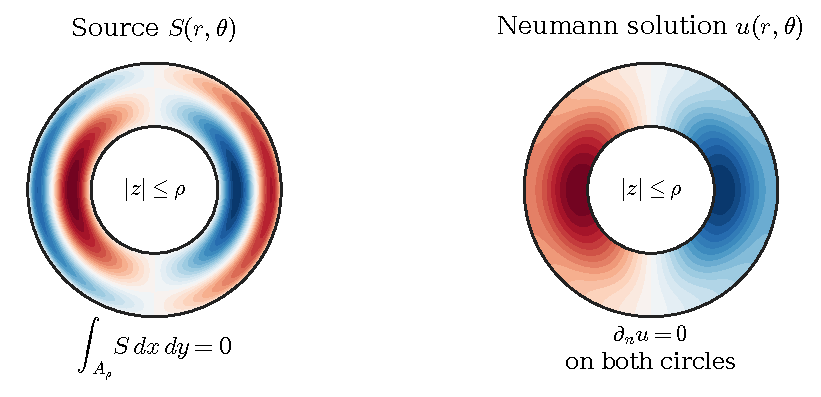
\includegraphics[width=\textwidth]{figures/output/fig06_neumann.pdf}
\caption{A scalar first-angular-mode example of the collar
construction, with colors normalized separately in the two panels.
For $x=r/\rho$, let $\chi(x)=6(x-1)^5-15(x-1)^4+10(x-1)^3$ and
$u=\rho(\chi(x)x-4x/3-4/(3x))\cos\theta$.
Then $S=-\Delta_{\RR^2}u$ has zero mean and $\partial_nu=0$
at $r=\rho,2\rho$. The matrix construction uses the same
compatibility condition and energy estimate; it does not require
this particular scalar source.}
\label{fig:neumann}
\end{figure}

Define $B=\cR(\widehat K)-D^*J$ on the whole fibre. The
component and middle-node estimates
\eqref{eq:component-residual}--\eqref{eq:transfer-residual},
the regular and radial collar estimates
\eqref{eq:regular-curvature-error}--\eqref{eq:radial-curvature-error},
and \eqref{eq:nonlinear-collar-remainder} now give
\begin{equation}\label{eq:instantaneous-b}
 \int_{C_\tau}|B|\le
 C(\alpha_*+\epsilon_*\ell^2+b^2\rho^{-N})(F+V).
\end{equation}
For the remaining Taylor terms use
$\alpha_i^2\rho^2m_i\le C\rho^2F_{\mathrm{co}}$ and
$\alpha_i^2\rho^2\ell F_{\mathrm{ed}}
\le C\alpha_*^2\rho^2\ell F_{\mathrm{ed}}$.
The time terms are bounded by $C\rho^2V$.
Thus no term weighted only by $|\alpha_i|m_i$ remains in
\eqref{eq:instantaneous-b}. Integrating
\eqref{eq:instantaneous-j} by the finite energy inequality and
\eqref{eq:instantaneous-b} by \eqref{eq:integrable-forces}
proves Proposition~\ref{prop:global-weak-residual}.

\subsection{The all-time theorem}
\begin{theorem}\label{thm:all-time}
Fix the component geometry, rank, harmonic forms, component matrices
and transports of Section~\ref{sec:geometry}. There is a radius
$R_*>0$ such that the following holds. Let the four nonzero node
parameters and the two real component parameters tend independently
to zero, and keep them fixed during each trajectory. Let $H(s)$
solve \eqref{eq:finite-flow} from $d_A(H(0),o)\le R_*$.
For any smooth determinant-normalized actual initial metric with
fixed bounds $ch_0\le h(0)\le C_0h_0$, let $h(s)$ solve HYM.
With $\widehat K$ as in Section~\ref{sec:reconstruction} and
$\eta=\int_{C_\tau}D_{\tr}(h(0),\widehat K(H(0)))$, one has
\begin{equation}\label{eq:all-time-tracking}
 \sup_{s\ge0}\int_{C_\tau}
       d(h(s),\widehat K(H(s)))^2\,dA_\tau
                     \le\eta+C a_* .
\end{equation}
The constant is independent of every scale ratio and of time.
The conclusion permits zero component weights and a nonzero
common kernel in \eqref{eq:common-kernel}. No positive lower
bound on a normalized smallest eigenvalue is assumed.
\end{theorem}

\begin{proof}
The actual flow is global and has the fixed order bounds by
\eqref{eq:order-bounds}. Its total derivative energy is bounded
by \eqref{eq:actual-energy}, since every fibre has area four.
Lemma~\ref{lem:reconstruction-energy} supplies the same bound
for the comparison. Apply Lemma~\ref{lem:weak-comparison} to the
global decomposition in Proposition~\ref{prop:global-weak-residual}.
Its right-hand side is at most $\eta+C(a_*+\rho)$, uniformly for
all finite time horizons. Since $\rho\le a_*$, taking the supremum
over horizons proves \eqref{eq:all-time-tracking}.
\end{proof}

Uniform convergence in a family of initial metrics requires
$\eta\to0$ uniformly in that family. The theorem compares each
parameter-dependent finite trajectory with its actual HYM
trajectory. It asserts neither a common limiting trajectory nor
a selected limiting phase in a nonzero kernel. When the active
constraints are irreducible, the finite limit is $o$; the theorem
still concerns absolute distance, not an error relative to the
decaying trajectory. The next section supplies an open spatial
class that enters this comparison after a negligible initial
time on every effective scale.

\section{Entry from spatially varying metrics}\label{sec:entry}

We specify an open class of initial metrics without prescribing their
finite initial tuple. The tuple is selected by auxiliary flows on
the fixed closed normalization components at $\alpha=0$. Their
use during a short preparation interval will be justified on the
actual smoothing.

\subsection{The selected constant metric on a fixed component}
Let $Y$ be a fixed connected closed Riemann surface of area $A$.
For matrix functions write $\langle f\rangle=A^{-1}\int_Y f\,dA$,
and let $\lambda_1>0$ be the first positive scalar eigenvalue.
Consider the trivial holomorphic bundle in a fixed global flat frame.

\begin{lemma}\label{lem:component-phase}
Let $h(s)$ be HYM flow from a smooth determinant-one metric with
$cI\le h(0)\le C_0I$. There is a unique constant determinant-one
matrix $P$ such that $h(s)\to P$ uniformly. With
$M(s)=\langle h(s)\rangle$, $J(s)=\log\det M(s)$ and
$W(s)=\langle\|h(s)-M(s)\|^2\rangle$, one has
\begin{equation}\label{eq:phase-estimates}
 \begin{gathered}
 M'(s)\preceq0,\qquad P=\lim_{s\to\infty}M(s),\qquad
 cI\le P\le C_0I,\\
 \frac{W}{2C_0^2}\le J\le\frac{W}{2c^2},\qquad
 J(s)\le J(0)e^{-\gamma s},\qquad
 \tr(M(s)-P)\le C_0J(s),\qquad
 \gamma=\frac{2c^2}{C_0^2}\lambda_1.
 \end{gathered}
\end{equation}
For $s\ge1$,
\begin{equation}\label{eq:phase-uniform}
 \sup_Y d(h(s),P)^2\le
 C_Y(2J(0)+J(0)^2)e^{-\gamma(s-1)}.
\end{equation}
If $P,P'$ are selected by two initial metrics in this bounded range,
then
\begin{equation}\label{eq:phase-contraction}
 A D_{\tr}(P,P')\le
          \int_Y D_{\tr}(h(0),h'(0))\,dA.
\end{equation}
Constants in these conclusions do not use derivatives of the
initial metrics.
\end{lemma}

\begin{proof}
Equation \eqref{eq:local-hym} is $h_s=-\Delta h-Q(h)$ with
$Q=4a^{-1}h_z^*h^{-1}h_z\succeq0$. Averaging gives
$M'=-\langle Q\rangle\preceq0$. The bounded decreasing
Hermitian family $M(s)$ has a limit $P$ with eigenvalues in
$[c,C_0]$; the determinant of this limit has not yet been
determined.

For $f(B)=\log\det B$ and a Hermitian matrix $Z$,
\[
 -D^2f_B[Z,Z]=\tr(B^{-1}ZB^{-1}Z),\qquad
 C_0^{-2}\|Z\|^2\le -D^2f_B[Z,Z]\le c^{-2}\|Z\|^2
\]
on the same matrix interval. Taylor's integral formula along the
segment from $M$ to $h(x)$, averaged over $Y$, has zero linear
term. Since $\log\det h(x)=0$, it gives the two bounds between
$J$ and $W$ in \eqref{eq:phase-estimates}.

Using $M^{-1}\ge C_0^{-1}I$, then $h^{-1}\ge C_0^{-1}I$,
gives
\[
 -J'=\tr(M^{-1}\langle Q\rangle)
       \ge C_0^{-1}\langle\tr Q\rangle
       \ge C_0^{-2}\langle|dh|^2\rangle.
\]
Here $4a^{-1}\tr(h_z^*h_z)=|dh|^2$. This identity takes the
trace before any nonconstant matrix weight is introduced; no
weighted commutator has been dropped. Applying the scalar
Poincar\'e inequality to the real matrix entries of $h-M$
gives $\langle|dh|^2\rangle\ge\lambda_1 W\ge2c^2\lambda_1J$.
This proves the exponential bound for $J$.

It follows that $\det P=1$. Since $M-P\succeq0$,
integration of the logarithmic determinant along the segment
from $P$ to $M$ gives
$J\ge C_0^{-1}\tr(M-P)$. The cross term vanishes when averaging
$\|h-P\|^2$, so
\[
 \langle\|h-P\|^2\rangle
    =W+\|M-P\|^2\le C_0^2(2J+J^2).
\]
This proves exponential $L^2$ convergence.

The constant $P$ is an exact stationary solution. By
Lemma~\ref{lem:forced-trace}, $D_{\tr}(h,P)$ is a scalar heat
subsolution. The time-one scalar heat kernel on this fixed
compact surface is bounded. Thus its supremum at $s\ge1$ is at
most a fixed multiple of its integral at $s-1$. Equivalence of
trace and squared matrix distances on the bounded range proves
\eqref{eq:phase-uniform}. Applying the integrated unforced trace
comparison to two flows and passing to their uniform limits
proves \eqref{eq:phase-contraction}.
\end{proof}

The selected matrix depends on the full initial metric. For
simultaneously diagonal data
$h(0)=\operatorname{diag}(e^{f_1},\ldots,e^{f_r})$ with
$\sum_a f_a=0$, the scalar heat equation gives
$P=\operatorname{diag}(e^{\langle f_1\rangle},\ldots,
e^{\langle f_r\rangle})$. In general neither the initial
arithmetic mean nor the exponential of its mean logarithm is
asserted to equal $P$.

\subsection{An open class on the smooth fibres}
Fix $0<\beta<1$. Let $\Omega_i(2\rho)$ be the closed component
with the branch disks of radius $2\rho$ removed, identified with
its region in the smooth fibre. For a smooth trace-free
$h_0$-Hermitian logarithm $S$, express its restriction $S_i$
in the harmonic component gauge and set
\begin{equation}\label{eq:extension-norm}
 \cN(S)=\|S\|_{C^0(C_\tau)}
  +\sum_i\inf_{\widetilde S_i|_{\Omega_i(2\rho)}=S_i}
                    \|\widetilde S_i\|_{C^{6,\beta}(C_i)}.
\end{equation}
Each infimum is over smooth Hermitian trace-free extensions
to the closed component $C_i$.
Define $\mathcal B_{R_0}=\{e^S:\cN(S)<R_0\}$. For each
fixed fibre this is an open nonempty class in the smooth
$C^{6,\beta}$ topology. Indeed restriction to the punctured
components has a bounded linear extension across their smooth
boundary circles, so each infimum seminorm is continuous.
No uniform estimate for this extension operator as
$\rho\to0$ is needed or claimed.

The class includes small smooth component profiles. It also
permits arbitrary smooth modifications inside the removed disks
and middle nodes, provided the global $C^0$ bound and strict
norm margin are preserved. In particular their spatial
derivatives there need not be uniformly bounded. Choose $R_0$
small enough that phases obtained from extensions with total
norm below $2R_0$ lie in the finite ball of
Theorem~\ref{thm:all-time}. This is possible because their
order bounds imply
$d_A(P,o)\le2\sqrt{r\sum_i A_i}\,R_0$.

\begin{theorem}\label{thm:spatial-entry}
For the fixed data of Theorem~\ref{thm:all-time} and sufficiently
small $R_0>0$, every initial metric in $\mathcal B_{R_0}$ has
a selected tuple $P$ and a common preparation time
$s_*\to\infty$ such that $\sigma s_*\to0$ and
\begin{equation}\label{eq:entry-trace}
 \eta_*:=\int_{C_\tau}
             D_{\tr}(h(s_*),\widehat K(P))\,dA_\tau\longrightarrow0.
\end{equation}
The time and convergence bounds are uniform over this class and
all permitted scale ratios. If $H_f(s)$ is the finite solution
with $H_f(0)=P$, then
\begin{equation}\label{eq:spatial-all-time}
 \sup_{s\ge s_*}\int_{C_\tau}
      d(h(s),\widehat K(H_f(s)))^2\,dA_\tau
 \le C\{\eta_*+a_*+(\sigma s_*)^2\}\longrightarrow0.
\end{equation}
Different admissible extensions in \eqref{eq:extension-norm}
give tuples at distance $O(\rho)$ and reconstructions at
integrated squared distance $O(\rho^2)$ at every later time.
\end{theorem}

\begin{proof}
Choose extensions $\widetilde S_i$ with total $C^{6,\beta}$
norm below $2R_0$. Let $\Psi_i(s)$ be HYM flow for the trivial
connection on the fixed closed component, from
$\exp(\widetilde S_i)$, and let $P_i$ be its phase from
Lemma~\ref{lem:component-phase}. These auxiliary flows have
$\alpha_i=0$. Their difference from the actual component
equation will be estimated explicitly.

For each integer $n\ge1$, fixed-component parabolic theory
gives a constant $C_n\ge1$ controlling two spatial derivatives
and one time derivative of all these flows on $[0,n]$.
One can choose $C_n$ nondecreasing. To justify uniformity over
the profiles, the bounded initial $C^{6,\beta}$ class is
precompact in $C^{4,\beta/2}$; continuous dependence for the
fixed strictly parabolic equation, the order bounds and
fixed-component continuation give a finite bound on each
finite time interval. No assertion that $C_n$ stays bounded
as $n\to\infty$ is used.

Construct a preparation metric $K_{\mathrm{pre}}(s)$ with
$\Psi_i(s)$ on $\Omega_i(2\rho)$. Use node geodesics between
their values at the branch points, with parameter
$-\epsilon_e\log|u_e|$, and interpolate relative logarithms
on the incidence collars, including the actual unitary
changes of frame. As before this is a global smooth
determinant-normalized metric with fixed order bounds.
On the component exterior, subtracting the trivial-connection
equation from the actual $D_i$ equation leaves integrated
error at most $C_n\alpha_*$. Metric transfer contributes
$C_n b^2\rho^{-N}$. The node curvature is zero and its time
residual has integral at most $C_n\rho^2$.

On an incidence collar the component value differs from its
value at the branch point by $O(C_n\rho)$, including the
change of frame. The node logarithm differs from that point
value by $O(C_n\epsilon_e|\log\rho|)$. The discrepancy
derivatives of order $k\le2$ are therefore bounded by
$C_n(\rho+\epsilon_*|\log\rho|)\rho^{-k}$. The full
curvature-difference estimate used in Section~\ref{sec:angular}
gives the integrated bound
$C_n(\rho+\epsilon_*|\log\rho|)$, with the quadratic terms
included. Consequently
\begin{equation}\label{eq:preparation-residual}
 \sup_{0\le s\le n}\int_{C_\tau}|\cR(K_{\mathrm{pre}}(s))|
       \le C_n\delta_*,
 \qquad
 \delta_*=\alpha_*+\epsilon_*\ell+b^2\rho^{-N}\to0.
\end{equation}
At time zero $K_{\mathrm{pre}}$ and $h(0)$ agree on every
$\Omega_i(2\rho)$ and have bounded difference elsewhere.
The latter region has area $O(\rho^2)$. Integrated forced
trace comparison gives error at most
$C\rho^2+C_nn\delta_*$ through time $n$.

For sufficiently small parameters choose
\begin{equation}\label{eq:preparation-time}
 s_*=\max\{n\in\mathbb N:nC_n\le\delta_*^{-1/2}\}.
\end{equation}
Then $s_*\to\infty$ and $\sigma s_*\to0$, since
$\sigma\le C\delta_*$. Uniform convergence of the auxiliary
flows to $P_i$, the component Green $L^2$ bounds, and the
area $O(\rho^2)$ of the remaining regions show
\begin{equation}\label{eq:quantitative-entry}
 \eta_*\le C\bigl(\sqrt{\delta_*}
                +e^{-\gamma_0(s_*-1)}+\epsilon_*^2\bigr)
                   \longrightarrow0
\end{equation}
for a fixed $\gamma_0>0$ depending on the component
geometries and initial order bounds. On this range trace
distance and squared affine distance are equivalent, so the
triangle comparison used here costs only a fixed constant.

Restart Theorem~\ref{thm:all-time} at $s_*$ from the finite
tuple $P$. This first compares $h(s)$ with
$\widehat K(H_f(s-s_*))$. Convex gradient flow on the
Hadamard product is nonexpanding: first variation of the
squared distance between two solutions and convexity make
its derivative nonpositive. Autonomy therefore gives
\[
 d_A(H_f(s-s_*),H_f(s))
       \le d_A(P,H_f(s_*))\le C\sigma s_*
       \qquad(s\ge s_*).
\]
Lemma~\ref{lem:reconstruction-energy} transfers this
difference to global integrated squared distance, proving
\eqref{eq:spatial-all-time}.

Two choices of extensions agree on $\Omega_i(2\rho)$.
Their initial component trace difference is bounded and
supported on disks of total area $O(\rho^2)$.
Equation \eqref{eq:phase-contraction} yields
$d_A(P,P')=O(\rho)$. Nonexpansion of finite flow and
\eqref{eq:reconstruction-lipschitz} preserve the asserted
ambiguity for all later times.
\end{proof}

The preparation time is negligible compared with every finite
scale: $\sigma s_*\to0$, while all finite speeds are bounded
by a constant times $\sigma$. No approximation is asserted
during the discarded initial layer. The tuple $P$ depends on
the spatial initial data; convergence to a single
parameter-independent finite trajectory would require
convergence of the selected phases and of the rescaled
parameters, in addition to the estimates proved here.

\section{The complete small spectrum and a three-scale family}\label{sec:spectrum}

The linearization of HYM at the parallel metric is the heat
equation for the induced connection Laplacian on trace-free
Hermitian endomorphisms. Write $\mathfrak p_r=\Herm_0(r)$,
$d=r^2-1$, $m=4d$, and
\[
 \mathcal L_{\tau,\alpha,U}=D^*D,\qquad
 \mathcal E_\tau(s)=\int_{C_\tau}|Ds|^2\,dA_\tau .
\]
In this section the unitary transports may vary between fibres.
For $X\in\mathfrak p_r^4$ set
\begin{equation}\label{eq:effective-forms}
 \begin{split}
 M(X)&=\sum_i A_i\|X_i\|^2,\\
 g_\alpha(X)&=\sum_{i=+,-}\alpha_i^2\kappa_i\|[T_i,X_i]\|^2,\\
 Q(X)&=g_\alpha(X)+
       \sum_{e=ij}w_e\|X_i-\Ad(U_{ij})X_j\|^2,\qquad
 w_e=2\pi/L_e .
 \end{split}
\end{equation}
These are respectively the mass form and the Hessian of
\eqref{eq:potential} at $o$. They are defined by the component
geometry, harmonic forms and node transports before solving a
global analytic problem.

\begin{theorem}\label{thm:relative-spectrum}
Let $\nu_0\le\cdots\le\nu_{m-1}$ be the generalized eigenvalues
of $(Q,M)$, including zeros, and let
$\lambda_0\le\lambda_1\le\cdots$ be those of
$\mathcal L_{\tau,\alpha,U}$. There are $\gamma>0$ and
$e(\alpha_*,b)\to0$ as $\alpha_*,b\to0$ such that
\begin{equation}\label{eq:relative-spectrum}
 (1-e)\nu_k\le\lambda_k\le(1+e)\nu_k\quad(0\le k<m),
 \qquad \lambda_m\ge\gamma.
\end{equation}
Exactly $m$ eigenvalues, counting zeros, tend to zero. The kernels
of the finite and actual operators correspond exactly through
\eqref{eq:common-kernel}. The estimates are uniform in all
$\alpha_i^2L_e$, all $L_e/L_f$, and all unitary transports,
including reducible ones.

Component averaging identifies the $m$-dimensional spectral
subspace associated with the eigenvalues tending to zero
asymptotically isometrically with $(\mathfrak p_r^4,M)$.
Let $\Pi$ be the orthogonal projection onto this small-eigenvalue
subspace, and let $P_a$ be the orthogonal projection onto the
image of the trial map $J_a$ constructed below. Then
\begin{equation}\label{eq:projection-comparison}
 \|\Pi-P_a\|_{L^2\to L^2}
                \le C\sqrt{\alpha_*^2+w_*},\qquad
 w_*=\max_e w_e.
\end{equation}
On the complementary space the inverse, heat and resolvent
bounds are respectively $\gamma^{-1}$, $e^{-\gamma s}$
and $(\gamma+\operatorname{Re}z)^{-1}$ for
$\operatorname{Re}z\ge0$.
\end{theorem}

The scalar graph approximation on degenerating surfaces has a
substantial history, including relative estimates with arbitrary
short-edge ratios \cite{burger}. Here the point requiring proof
is the combined component-and-node estimate, including the
commutator kernel and every weaker positive scale.

\subsection{Trial sections}
Choose a small fixed radius $a$ in the branch disks, independent
of all degenerating parameters. On an elliptic component begin
with the constant matrix $X_i$ in the harmonic gauge. On
$a<|u|<2a$ interpolate it with its parallel extension having
node value $X_i$. The primitive of the harmonic one-form obeys
$|F_{ie}|\le Ca$ and $|dF_{ie}|\le C$. The exact bound
\[
 \|\Ad(e^{i\alpha_iT_iF_{ie}})X_i-X_i\|
           \le|\alpha_iF_{ie}|\|[T_i,X_i]\|
\]
retains the component energy factor in every cutoff term.
The component energy is at most $(1+Ca^2)g_\alpha(X)$.
On rational components use constants. Conformal invariance
transfers these energies to the fibre exactly.

On the remaining node annulus, whose conformal length is
$\ell_e=L_e+2\log a$, interpolate the two parallel-frame
values affinely in logarithmic radius. Its energy is exactly
$(2\pi/\ell_e)\|X_i-\Ad(U_e)X_j\|^2$. Denote the resulting
continuous $H^1$ trial section by $J_aX$. Then
\begin{equation}\label{eq:trial-estimates}
 \begin{split}
 \mathcal E_\tau(J_aX)&\le(1+Ca^2)g_\alpha(X)
       +\sum_e\frac{2\pi}{\ell_e}
                      \|X_i-\Ad(U_e)X_j\|^2,\\
 1\le L_e/\ell_e&\le1+C_a/L_*,\\
 \bigl|\|J_aX\|_{L^2}^2-M(X)\bigr|
       &\le(Ca^2+o_a(b))M(X).
 \end{split}
\end{equation}
The mass estimate uses the $O(a^2)$ disk and annular areas,
unitarity and bounded interpolation, and smooth metric
convergence on fixed component exteriors. It is uniform in
the transports and length ratios. Min--max gives the relative
upper bound in \eqref{eq:relative-spectrum}, first choosing
$a$ small and then the parameters small. For one fixed $a$
it also gives $\lambda_{m-1}\le C(\alpha_*^2+w_*)$.

\subsection{Component means with an energy-controlled frame error}
On the punctured elliptic domain $\Omega_i(a)$, let
$\vartheta_{i,a}$ be the absolute harmonic representative of
the restriction class of $\vartheta_i$, with zero normal
component at the boundary. Write
$\vartheta_i=\vartheta_{i,a}+df_{i,a}$ and
$\kappa_{i,a}=\|\vartheta_{i,a}\|_{L^2}^2$.
Then $\kappa_{i,a}\to\kappa_i>0$. For completeness, the
restriction of $\vartheta_i$ is a competitor for the energy
minimization, giving a uniform upper bound. A weakly
convergent harmonic subsequence on compact subsets has finite
$L^2$ energy across every puncture. Its holomorphic
representation has no negative Laurent terms with finite
$L^2$ norm, so it extends across the puncture. Its periods,
including zero puncture periods, are those of
$\vartheta_i$. Uniqueness of the harmonic representative
on the closed component and lower semicontinuity prove
the asserted norm convergence.

Gauge by $e^{i\alpha_iT_if_{i,a}}$ and diagonalize $T_i$.
Each matrix entry then has connection
$d-i\beta\vartheta_{i,a}$ with
$\beta=\alpha_i(t_b-t_c)$. Decompose an entry as $v=z+w$,
where $w$ has mean zero. Coclosedness and the zero normal
condition give
$\langle dw,\vartheta_{i,a}z\rangle=0$.
The fixed-domain Poincar\'e inequality and a small-$\beta$
perturbation give
$\|w\|\le C_a\|(d-i\beta\vartheta_{i,a})w\|$.
The remaining cross term is bounded by
$C_a\beta^2|z|\|w\|$. Completing the square therefore yields
\begin{equation}\label{eq:component-lower-entry}
 \|(d-i\beta\vartheta_{i,a})v\|^2
 \ge\frac12\|(d-i\beta\vartheta_{i,a})w\|^2
            +(\beta^2\kappa_{i,a}-C_a\beta^4)|z|^2.
\end{equation}
Summing matrix entries defines a real linear average
$s\mapsto X_i(s)$ and gives
\begin{equation}\label{eq:component-lower}
 \begin{split}
 \mathcal E_i(s)&\ge
   (1-C_a\alpha_*^2)\alpha_i^2\kappa_{i,a}
                                  \|[T_i,X_i]\|^2,\\
 \|w_i\|_{H^1}^2+\alpha_i^2\|[T_i,X_i]\|^2
                                      &\le C_a\mathcal E_i(s).
 \end{split}
\end{equation}
No division by $\alpha_i$ or an eigenvalue difference is used.
On rational components take the ordinary mean. These estimates
concern actual component energy by conformal invariance.

Let $c_{ie}$ be the boundary-circle mean in the parallel node
frame. The change from the averaging gauge to this frame
acting on $X_i$ is at most
$C_a|\alpha_i|\|[T_i,X_i]\|$. The remaining error is bounded
by the $H^1$ trace norm of $w_i$. Thus
\begin{equation}\label{eq:boundary-means}
 \|c_{ie}-X_i(s)\|\le C_a\mathcal E_i(s)^{1/2}.
\end{equation}
Replacing this by an error proportional to
$|\alpha_i|\|X_i\|$ would lose relative control near a
changing commutant.

\subsection{The combined lower form}
Partition the energy into the disjoint truncated components
and their complementary node annuli:
$\mathcal E_\tau=\mathcal E_{\mathrm{comp}}
                  +\mathcal E_{\mathrm{neck}}$.
Angular averaging and the one-dimensional Dirichlet principle
give
\[
 \sum_e\frac{2\pi}{\ell_e}
       \|c_{ie}-\Ad(U_e)c_{je}\|^2
                   \le\mathcal E_{\mathrm{neck}}.
\]
Apply the triangle inequality in the direct sum of edge
spaces weighted by $\sqrt{w_e}$. Using
$w_e\le2\pi/\ell_e$ and \eqref{eq:boundary-means} gives
\begin{equation}\label{eq:weighted-neck-lower}
 \left(\sum_e w_e\|X_i-\Ad(U_e)X_j\|^2\right)^{1/2}
 \le\mathcal E_{\mathrm{neck}}^{1/2}
           +C_a\sqrt{w_*}\,\mathcal E_{\mathrm{comp}}^{1/2}.
\end{equation}
With $\delta=C_a\sqrt{w_*}$ use
$(x+\delta y)^2\le(1+\delta)x^2+(\delta+\delta^2)y^2$.
Meanwhile \eqref{eq:component-lower} and
$\kappa_{i,a}\to\kappa_i$ give
$g_\alpha(X)\le(1+\theta(a)+C_a\alpha_*^2)
                   \mathcal E_{\mathrm{comp}}$, where
$\theta(a)\to0$. Adding the two estimates yields
\begin{equation}\label{eq:combined-form-lower}
 Q(X(s))\le
   \{1+\theta(a)+C_a\alpha_*^2+O_a(\sqrt{w_*})\}
                                    \mathcal E_\tau(s).
\end{equation}
The component and annular energies have not been counted
twice. This estimate is relative to their actual sum and
contains no smallest scale in a denominator.

\subsection{Mass and completeness}
We give the mass estimate needed both for the lower eigenvalue
bound and for completeness of the mode list. Let $s$ be a unit
eigensection with eigenvalue $\lambda\le1$. Equation
\eqref{eq:component-lower} bounds its mean-zero component
parts in $H^1$ by $C_a\sqrt\lambda$. On fixed collars,
interior elliptic estimates improve the boundary error to
the same order in supremum norm. In the equation for the
mean-zero part, the Laplacian of the gauged constant is
$\alpha_i^2|\vartheta_{i,a}|^2\operatorname{ad}(T_i)^2X_i$.
Its norm is bounded by $C_a|\alpha_i|\sqrt{\mathcal E_i}$
using \eqref{eq:component-lower}. The other inhomogeneous
term is $\lambda s$. Enlarge the fixed collar across the
circle before applying the interior estimate. In the
actual conformal metric the connection Laplacian is
multiplied by a bounded smooth scalar there, without a new
first-order term. The leading boundary values have size
at most $C\|X_i\|$ with $C$ independent of $a$, because
the changes of frame are unitary.

On each node annulus split the section into its entrywise
harmonic Dirichlet extension $h$ and a zero-boundary remainder
$v$. The maximum principle and annular area $O(a^2)$ bound
the mass of $h$ by $Ca^2+C_a\sqrt\lambda$. Orthogonality
of Dirichlet energies gives
$\mathcal E(v)\le\mathcal E(s)$. The zero-boundary Poincar\'e
estimate
\begin{equation}\label{eq:annulus-poincare}
 \|v\|_{L^2(dA_\tau)}^2\le Ca^2\mathcal E(v)
\end{equation}
is uniform in the annular modulus. To verify it, the
metric is bounded by a fixed multiple of
$|du|^2+|dv_{\mathrm{branch}}|^2$, with
$v_{\mathrm{branch}}=\tau_e/u$. For the first branch,
the zero outer boundary value and radial Cauchy--Schwarz
give
$|v(r,\theta)|^2\le\log(a/r)\int_r^a
|\partial_tv(t,\theta)|^2t\,dt$.
Integration against $r\,dr\,d\theta$ is bounded by
$Ca^2$ times the radial energy. The other branch gives
the same estimate for its area term, using the zero
boundary value at its outer circle. This proves
\eqref{eq:annulus-poincare}.

The component mean decomposition, metric convergence on
fixed exteriors, and these annular bounds now imply that
on any span of at most $m+1$ orthonormal eigensections
with eigenvalues at most $\Lambda\le1$,
\begin{equation}\label{eq:weak-mass}
 |M(X(s))-\|s\|_{L^2}^2|
 \le\{Ca^2+C_a\sqrt\Lambda+o_a(b)\}\|s\|_{L^2}^2.
\end{equation}
Passing from individual eigensections to this span costs
only its fixed dimension. The leading omitted-area
constant is independent of $a$.

If $\lambda_m$ tended to zero along a joint degeneration,
first choose $a$ small and then take the parameters far
along that sequence. Equation \eqref{eq:weak-mass} would
make averaging injective on an $(m+1)$-dimensional space
into $\mathfrak p_r^4$, a contradiction. This proves
the uniform complementary gap. The trial upper bound
already puts $m$ eigenvalues below it.

For the first $k+1$ eigensections use
$\Lambda=C(\alpha_*^2+w_*)$ in \eqref{eq:weak-mass}.
Their averages form a $(k+1)$-dimensional space.
Finite min--max gives a section in this span with
$Q(X(s))\ge\nu_kM(X(s))$. Combining this with
\eqref{eq:combined-form-lower} proves the relative lower
bound. For any requested error first choose $a$, then
choose $\alpha_*,b$ independently small. These quantifiers
give the function $e(\alpha_*,b)\to0$ in the theorem,
uniformly in all remaining ratios and transports.

The zero set of $Q$ is exactly
\eqref{eq:common-kernel}, since every node weight is
positive. Section~\ref{sec:geometry} identifies these
tuples with all global parallel endomorphisms, which are
precisely the kernel of $D^*D$. Thus zeros agree exactly
through all kernel changes.

Choose $a=a(\alpha_*,b)$ tending sufficiently slowly to
zero that the preceding errors vanish and
$|\log a|/L_*\to0$. The averaging and trial mass
estimates are then asymptotic isometries. On the
complement of the small-eigenvalue subspace, the gap gives
\[
 \|(1-\Pi)J_aX\|^2\le
       \gamma^{-1}\mathcal E_\tau(J_aX)
       \le C(\alpha_*^2+w_*)M(X).
\]
The spaces have equal dimension and the trial mass
has a uniform lower bound. Equality of their maximal
principal angle with the norm of the difference of
orthogonal projections proves
\eqref{eq:projection-comparison}. The spectral theorem
gives the stated inverse, heat and resolvent estimates
on the complement. On the positive small-eigenvalue subspace the
smallest rate and inverse norm instead have the
relative comparison with the smallest positive
$\nu_k$; they need not stay bounded away from zero
and infinity. This completes the proof of
Theorem~\ref{thm:relative-spectrum}.

\subsection{A three-scale family}
Order the vertices as $E_+,R_p,E_-,R_q$, numbered $0,1,2,3$.
Use identity transports on $0$--$1$--$2$--$3$ and
$U=(I+i\sigma_x)/\sqrt2$ on $3$--$0$. Set $T_+=\sigma_z$,
$\alpha_-=0$, and, for $h>0$, take
\begin{equation}\label{eq:h-family}
 w_{01}=w_{12}=w_{23}=h,\quad w_{30}=h^2,\quad
 \alpha_+=h^2/\sqrt{\kappa_+},\quad
 \tau_e=\exp(-2\pi/w_e).
\end{equation}
These are genuine parameters of the compact family.
Section~\ref{sec:geometry} proves stability for all
sufficiently small $h>0$.

In the Hilbert--Schmidt orthonormal Pauli basis
$(\sigma_x,\sigma_y,\sigma_z)/\sqrt2$ at each vertex,
$M=I$ and the matrix of $Q$ is
\begin{equation}\label{eq:h-matrix}
 Q_h=h(L_{P_4}\otimes I_3)+h^2D_{30}^TD_{30}
          +h^4\operatorname{diag}(4,4,0,0,\ldots,0),
\end{equation}
where
\[
 L_{P_4}=\begin{pmatrix}
 1&-1&0&0\\-1&2&-1&0\\0&-1&2&-1\\0&0&-1&1
 \end{pmatrix},\qquad
 D_{30}X=X_3-RX_0,\qquad
 R=\begin{pmatrix}1&0&0\\0&0&1\\0&-1&0\end{pmatrix}.
\]
The positive path eigenvalues are $2-\sqrt2,2,2+\sqrt2$.
Thus nine finite eigenvalues are these three coefficients
times $h$, each with multiplicity three, up to $O(h^2)$.
The isometric constant-tuple inclusion
$Z\mapsto(Z,Z,Z,Z)/2$ compresses the cycle term to
$\operatorname{diag}(0,\tfrac12,\tfrac12)$ and the
component term to $\operatorname{diag}(1,1,0)$.
Schur complementation across the order-$h$ complement
therefore gives two eigenvalues
$\tfrac12h^2+O(h^3)$.

For the last eigenvalue one must use its invariant sector,
rather than this absolute remainder. The $\sigma_x$
sector is invariant, its graph operator has exact
constant kernel, and its positive gap is at least
$(2-\sqrt2)h$. The order-$h^4$ perturbation has
expectation $h^4$ on its unit constant vector.
The complementary inverse bound gives the last
eigenvalue $h^4+O(h^7)$. As a check on the displayed
finite matrix, its determinant is
\begin{equation}\label{eq:h-determinant}
 \det Q_h=16h^{17}(1+3h)(1+2h^2+6h^3).
\end{equation}
All entries and the compressions used in this calculation
are printed above.

\begin{corollary}\label{cor:three-scales}
On the stable compact family \eqref{eq:h-family}, nine
actual eigenvalues have leading coefficients
$2-\sqrt2,2,2+\sqrt2$, each three times, at order $h$;
two are asymptotic to $\tfrac12h^2$; one is
asymptotic to $h^4$. The next eigenvalue has a uniform
positive lower bound. On the fixed small basin of
Theorem~\ref{thm:all-time}, actual nonlinear HYM
trajectories are approximated by
\eqref{eq:finite-flow} through time $h^{-4}$ and all
later times, with absolute integrated squared-distance
error at most
$\eta+O(h(1+|\log h|)^2)$. The spatial initial class
of Theorem~\ref{thm:spatial-entry} has the corresponding
all-time conclusion after preparation.
\end{corollary}

\begin{proof}
Apply Theorem~\ref{thm:relative-spectrum} to the finite
eigenvalue estimates. Apply Theorems~\ref{thm:all-time}
and \ref{thm:spatial-entry} separately to the same
fixed matrices and transports. Here
$\epsilon_*=h/(2\pi)$, $\alpha_*=h^2/\sqrt{\kappa_+}$,
and $b=e^{-2\pi/h}$, so
$a_*=O(h(1+|\log h|)^2)$. The nonlinear conclusion
follows from the residual and energy proof, not from
the eigenvalue asymptotics.
\end{proof}

\section{Further questions}\label{sec:further}

The spectral comparison is uniform when the transports change,
whereas the all-time force estimate fixes their constraint spaces.
The counterexample in Section~\ref{sec:finite} identifies the
failure of one proof estimate, not a failure of HYM tracking.
An extension through varying transports would require a stronger
estimate for the residual or a comparison that avoids the separate
force integral. The energy comparison itself has no such
fixed-transport restriction.

The small finite basin is also a restriction of the force
argument. Convexity confines trajectories from arbitrary bounded
finite balls, and the exact HYM flow has global order bounds.
Neither fact by itself supplies the uniform separate-force
estimate on those larger balls. A global version of that estimate,
or another integrability mechanism, would enlarge the spatial
initial class.

Our bundle family is flat unitary and therefore polystable on
every smooth fibre. The stable-to-strictly-polystable transition
is genuine, but the construction contains no unstable or
nonunitary stratum. It has a locally free bundle on the smooth
total space and no concentration of curvature in the parallel
reference metrics. Singular graded quotients and bubbling would
introduce local concentration data not present in this model.

Finally, the all-time error is absolute. At reducible parameters
the finite trajectory can tend to a nonidentity parallel tuple,
and its phase is selected by the initial metric. A uniform
infinite-time limit over degenerating parameters is a different
question from uniform approximation of these individual
trajectories. The present theorem concerns metrics on bundle
fibres. Extending it to distances on the moduli space of bundles,
or to a higher-dimensional degenerating base, requires additional
geometric and analytic arguments.

\begin{thebibliography}{HKKP18}
\bibitem[Bur90]{burger}
M.~Burger, \emph{Small eigenvalues of Riemann surfaces and graphs},
Math. Z. \textbf{205} (1990), 395--420.
\href{https://doi.org/10.1007/BF02571252}{doi:10.1007/BF02571252}.

\bibitem[DW00]{dw}
G.~D.~Daskalopoulos and R.~A.~Wentworth,
\emph{The Yang--Mills flow near the boundary of Teichm\"uller space},
Math. Ann. \textbf{318} (2000), no.~1, 1--42.
\href{https://doi.org/10.1007/s002080000098}{doi:10.1007/s002080000098}.

\bibitem[Don85]{donaldson}
S.~K.~Donaldson,
\emph{Anti self-dual Yang--Mills connections over complex algebraic surfaces and stable vector bundles},
Proc. London Math. Soc. (3) \textbf{50} (1985), no.~1, 1--26.
\href{https://doi.org/10.1112/plms/s3-50.1.1}{doi:10.1112/plms/s3-50.1.1}.

\bibitem[HKKP18]{hkkp}
F.~Haiden, L.~Katzarkov, M.~Kontsevich and P.~Pandit,
\emph{Iterated logarithms and gradient flows}, preprint, 2018.
\href{https://arxiv.org/abs/1802.04123v1}{arXiv:1802.04123v1}.

\bibitem[HK14]{hubbard-koch}
J.~H.~Hubbard and S.~Koch,
\emph{An analytic construction of the Deligne--Mumford compactification of the moduli space of curves},
J. Differential Geom. \textbf{98} (2014), no.~2, 261--313.
\href{https://doi.org/10.4310/jdg/1406552251}{doi:10.4310/jdg/1406552251}.
\href{https://arxiv.org/abs/1301.0062v1}{arXiv:1301.0062v1}.

\bibitem[JW92]{ji-wentworth}
L.~Ji and R.~Wentworth, \emph{Spectral convergence on degenerating surfaces},
Duke Math. J. \textbf{66} (1992), no.~3, 469--501.
\href{https://doi.org/10.1215/S0012-7094-92-06615-4}{doi:10.1215/S0012-7094-92-06615-4}.

\bibitem[JW97]{ji-wentworth-correction}
L.~Ji and R.~Wentworth, \emph{Correction to \textquotedblleft Spectral convergence on degenerating surfaces\textquotedblright},
Duke Math. J. \textbf{90} (1997), no.~1, 205--207.
\href{https://doi.org/10.1215/S0012-7094-97-09007-4}{doi:10.1215/S0012-7094-97-09007-4}.

\bibitem[Kob87]{kobayashi}
S.~Kobayashi, \emph{Differential Geometry of Complex Vector Bundles},
Publ. Math. Soc. Japan \textbf{15}, Kan\^o Memorial Lectures \textbf{5},
Iwanami Shoten and Princeton University Press, 1987.
\href{https://www.mathsoc.jp/assets/pdf/publications/pubmsj/Vol15.pdf}{Authorized 2013 retypesetting}.

\bibitem[Lam26]{lam}
S.~T.~Lam, \emph{Semistability and asymptotics of geometric flows},
preprint, 2026.
\href{https://arxiv.org/abs/2606.09235v1}{arXiv:2606.09235v1}.

\bibitem[NS65]{narasimhan-seshadri}
M.~S.~Narasimhan and C.~S.~Seshadri,
\emph{Stable and unitary vector bundles on a compact Riemann surface},
Ann. of Math. (2) \textbf{82} (1965), no.~3, 540--567.
\href{https://doi.org/10.2307/1970710}{doi:10.2307/1970710}.

\bibitem[Oht20]{ohta}
S.~Ohta, \emph{Self-contracted curves in CAT(0)-spaces and their rectifiability},
J. Geom. Anal. \textbf{30} (2020), 936--967.
\href{https://doi.org/10.1007/s12220-018-00126-7}{doi:10.1007/s12220-018-00126-7}.
Theorem and equation numbering follows
\href{https://arxiv.org/abs/1711.09284v2}{arXiv:1711.09284v2}.

\bibitem[Wue26a]{wuebben-effective}
B.~J.~Wuebben,
\emph{Effective Hermitian--Yang--Mills flow on nodal degenerations of curves},
preprint, 10 November 2026.
\href{https://doi.org/10.5281/zenodo.24120966}{doi:10.5281/zenodo.24120966}.

\bibitem[Wue26b]{wuebben-gluing}
B.~J.~Wuebben,
\emph{Hermitian--Yang--Mills flow and gluing on degenerating curves},
preprint, 11 November 2026.
\href{https://doi.org/10.5281/zenodo.24149197}{doi:10.5281/zenodo.24149197}.
\end{thebibliography}

\end{document}
